\documentclass[a4paper, 7pt, landscape]{scrartcl}
\usepackage[german]{babel}
\usepackage[utf8]{inputenc}
\usepackage{multicol}
\usepackage{geometry}
\usepackage{graphicx}
\usepackage{wrapfig}
\usepackage{enumitem}
\usepackage{fancyhdr}
\usepackage{index}
\usepackage{sectsty}
\usepackage{mwe}
\usepackage{comment}
\usepackage{lipsum}
\usepackage{titlesec}
\usepackage[dvipsnames]{xcolor}
\usepackage{amsmath}
\usepackage{amssymb}


%Define Math Commands:
\newcommand*{\field}[1]{\mathbb{#1}}%
\newcommand{\Mod}[1]{\ (\mathrm{mod}\ #1)}

%Image Folder:
\graphicspath{{../img/}}

%format
\geometry{top=0.4cm,left=0.5cm,right=0.5cm,bottom=0.4cm}
\setlist{topsep=0pt, leftmargin=5mm, nolistsep}

% Code Snippets
\usepackage{courier} %% Sets font for listing as Courier.
\usepackage{listings}
\usepackage{graphicx}
\usepackage{graphicx}
\usepackage{graphicx}
\usepackage{graphicx}
\usepackage{graphicx}
\usepackage{graphicx}
\usepackage{graphicx}
\usepackage{graphicx}
\usepackage{graphicx}
\usepackage{graphicx}
\usepackage{graphicx}
\usepackage{graphicx}
\usepackage{graphicx}
\usepackage{graphicx}
\usepackage{graphicx}
\usepackage{listings}
\usepackage{graphicx}
\usepackage{graphicx}
\usepackage{graphicx}
\usepackage{graphicx}
\usepackage{graphicx}
\usepackage{graphicx}
\usepackage{graphicx}
\usepackage{graphicx}
\usepackage{graphicx}
\usepackage{graphicx}
\usepackage{graphicx}
\usepackage{graphicx}
\usepackage{graphicx}
\usepackage{graphicx}
\usepackage{graphicx}
\usepackage{graphicx}
\usepackage{graphicx}
\usepackage{graphicx}
\usepackage{graphicx}
\usepackage{graphicx}
\usepackage{graphicx}
\usepackage{graphicx}
\usepackage{graphicx}
\usepackage{graphicx}
\usepackage{graphicx}

\definecolor{javared}{rgb}{0.6,0,0} % for strings

%define Javascript language
\lstdefinelanguage{JavaScript}{
keywords={typeof, new, true, false, catch, function, return, null, catch, switch, var, if, in, while, do, else, case, break, const, let, var, console, log},
keywordstyle=\color{blue}\bfseries,
ndkeywords={class, export, boolean, throw, implements, import, this},
ndkeywordstyle=\color{darkgray}\bfseries,
identifierstyle=\color{black},
sensitive=false,
comment=[l]{//},
morecomment=[s]{/*}{*/},
commentstyle=\color{purple}\ttfamily,
stringstyle=\color{red}\ttfamily,
morestring=[b]',
morestring=[b]"
}

\lstset{
language=JavaScript,
basicstyle=\fontsize{7}{7} \ttfamily,
keywordstyle=\bfseries\color{RoyalBlue},
stringstyle=\color{javared},
commentstyle=\color{MidnightBlue},
morecomment=[s][\color{MidnightBlue}]{/**}{*/},
tabsize=2,
showspaces=false,
showstringspaces=false,
texcl = true,
rulecolor = \color{black},
breaklines = true,
aboveskip = 0.5em,
belowskip = 0.5em
}




% Define Section Format
\titleformat{name=\section}[block]
{\sffamily\normalsize}
{}
{0pt}
{\colorsection}
\titlespacing*{\section}{0pt}{0pt}{0pt}

\newcommand{\colorsection}[1]{%
\colorbox{MidnightBlue!40}{\parbox{0.98\linewidth}{\color{black}\thesection\ #1}}}


% Define Subsection Format
\titleformat{name=\subsection}[block]
{\sffamily\small}
{}
{0pt}
{\colorsubsection}
\titlespacing*{\subsection}{0pt}{0pt}{0pt}

\newcommand{\colorsubsection}[1]{%
\colorbox{YellowGreen!50}{\parbox{0.98\linewidth}{\color{black}\thesubsection\ #1}}}

% Define SubSubsection Format
\titleformat{name=\subsubsection}[block]
{\sffamily\small}
{}
{0pt}
{\colorsubsubsection}
\titlespacing*{\subsubsection}{0pt}{0pt}{0pt}

\newcommand{\colorsubsubsection}[1]{%
\colorbox{Goldenrod!50}{\parbox{0.98\linewidth}{\color{black}\thesubsubsection\ #1}}}


% -----------------------------------------------------------------------
\begin{document}
    %	\pagecolor{p}
    %	\color{t}
    \setlength{\columnseprule}{0.4pt}
    \footnotesize
    \begin{multicols*}{3}

        \input{../content/01_Introduction.tex}
        \usepackage{graphicx}
%! Author = Philipp Emmenegger
%! Date = 08/06/2021

\section{Processes}
\subsection{1st Generation - Waterfall}
\begin{itemize}
    \item Split up development in independent steps
    \item Use specialized teams for every step
    \item Noticeable success rate for simple problems
\end{itemize}
\subsection{Problems}
\subsubsection{Software is rarely simple}
\begin{itemize}
    \item Simple problems are candidates for waterfall
    \item Chaotic problems are best avoided
    \item Complicated or Complex problems ask for more appropriate processes
\end{itemize}
\subsubsection{Too much uncertainty}
\begin{itemize}
    \item Giving reliable estimates at the beginning of a project is near impossible
    \item Uncertainty decreases over time
    \item Waterfall does not incorporate learning
\end{itemize}
\subsubsection{Lack of feedback}
\begin{itemize}
    \item Early changes are inexpensive
    \item Fast feedback is favorable
    \item Waterfall has no feedback cycles
    \item Problems might be detected very late
\end{itemize}
\subsubsection{No parallelization}
\begin{itemize}
    \item Sequential work is slow
    \item Parallelization should be strived
\end{itemize}
\subsubsection{Unused features}
\begin{itemize}
    \item Customers want features they rarely or never use
    \item Reasons: missing feedback cycles and lack of prioritization
\end{itemize}
\subsubsection{Knowledge loss on handovers}
\subsubsection{Missing autonomy}
\begin{itemize}
    \item Specialists get bored
    \item They rarely feel attached to the product
    \item Negative impact on the quality
\end{itemize}
\subsubsection{Sacrificing Quality}
\begin{itemize}
    \item Reducing efforts in implementation / testing to save time
    \item other phases already completed
\end{itemize}

\subsection{2nd Generation - Iterative and incremental}
\begin{itemize}
    \item Plan on different levels
    \item Do a little of everything at all time
    \item Incororate fast feedback
    \item Deliver working software after every iteration
    \item Enable cross-functional teams
\end{itemize}
\subsubsection{Main Criticism}
\begin{itemize}
    \item Too many documents
    \item Too complex process model
    \item missing tailoring
\end{itemize}

\subsection{3rd Generation - Agile Development}
\begin{itemize}
    \item Keep the benefits from 2nd generation
    \item Make processes slim and flexible
    \item Focus on delivering working software
\end{itemize}

\subsubsection{Agile Manifesto}
\begin{itemize}
    \item Individuals and interactions over processes and tools
    \item Working software over comprehensive documentation
    \item Customer collaboration over contract negotiation
    \item Responding to change over following a plan
\end{itemize}

\subsubsection{Core Principles}
\begin{itemize}
    \item Development is incremental
    \item Development is iterative
    \item Perform activities parallel
    \item Roles blur
    \item Planning is adaptive
    \item Scope can vary
    \item Requirements can change
    \item Working software as primary measure
    \item Document as you go
\end{itemize}

\subsubsection{Delivering working software}
\begin{itemize}
    \item An MVP has enough value that people are willing to use / buy it
    \item Demonstrates enough future benefit
    \item Provides feedback loop
    \item Prioritizing the backlog accordingly
    \item Creating MVP = creating vertical slices
    \item Every iteration, extend the previous slice further
    \item Cross-functional teams are best suited
    \item Reduces technical risks
\end{itemize}

\subsection{Scrum}
\textbf{Scrum Team}
\begin{itemize}
    \item Developers
    \item Product Owner
    \begin{itemize}
        \item Accountable for maximizing the value from the work of the team
        \item Accountable for effective Product Backlog management / prioritization
    \end{itemize}
    \item Scrum Master
    \begin{itemize}
        \item Accountable for establishing Scrum
        \item Accountable for the teams effectiveness
    \end{itemize}
\end{itemize}
\textbf{Scrum Events}
\begin{itemize}
    \item The Sprint (fixed length - one month or less)
    \item Sprint Planning
    \begin{itemize}
        \item Define a sprint goal
        \item Select items from the product backlog
        \item Decompose selected items into smaller work items
    \end{itemize}
    \item Daily Scrum
    \item Sprint Review
    \item Sprint Retrospective
\end{itemize}
\textbf{Scrum Artifacts}
\begin{itemize}
    \item Product Backlog
    \item Sprint Backlog
    \item Increment
\end{itemize}
\textbf{Scrum Values}
\begin{itemize}
    \item Commitment
    \item Focus
    \item Openness
    \item Respect Courage
\end{itemize}

\subsubsection{Measure Progress}
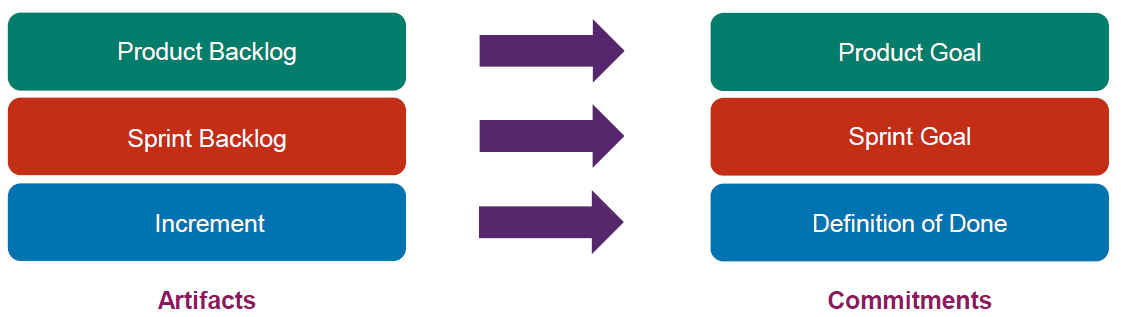
\includegraphics[width=\linewidth]{../img/scrum_progress.png}
        %! Author = Philipp Emmenegger
%! Date = 08/06/2021

\section{Backlog Management}
\subsection{User Stories}
\begin{itemize}
    \item Informal description from the perspective of a user
    \item May be written by anyone
\end{itemize}

\subsection{Tasks}
\begin{itemize}
    \item Work items
    \item Created as part of the Sprint Planning / Refinement meeting
    \item Be specific
    \item Should be small
    \item Assign categories
    \item Use a workflow
    \item Track real efforts
\end{itemize}

\subsection{Epics}
\begin{itemize}
    \item Rough description of something that might be needed in the future
    \item Same format as User Stories, omit details not yet needed
\end{itemize}

\subsection{Refinement Meeting}
\begin{itemize}
    \item Refine the product backlog with the whole scrum team
    \item Keep the backlog in a good shape
    \item No official Scrum event
\end{itemize}

\subsection{Story Maps}
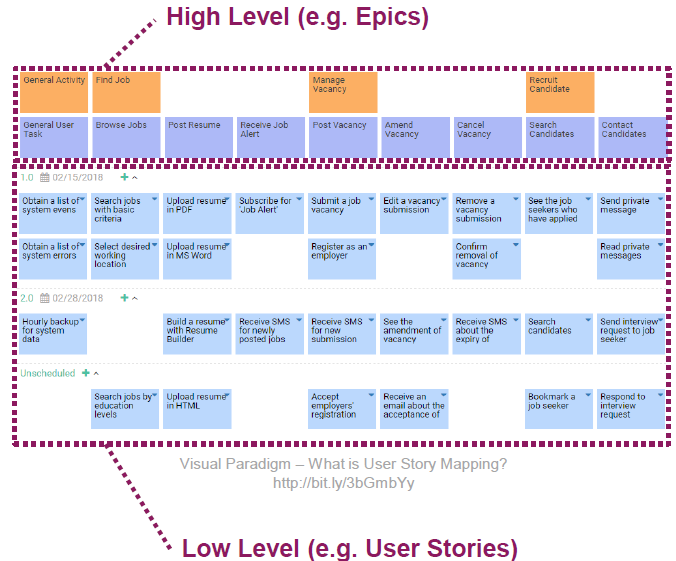
\includegraphics[width=\linewidth]{../img/story_maps.png}
\begin{itemize}
    \item Sort by activity horizontally
    \item Sort by priority vertically
    \item Usefull for release planning (MVP functionality)
    \item Can be used to create an initial backlog
\end{itemize}

\subsection{Release Planning}
\textbf{Requirements}
\begin{itemize}
    \item Estimates for all required functionality
    \item Velocity of the team
\end{itemize}
\textbf{Estimates}
\begin{itemize}
    \item Can be made in Refinements
\end{itemize}
\textbf{Velocity}
\begin{itemize}
    \item best measured in iterations
    \item can only be measured after executing some iterations
    \item otherwise use estimates / historical data
    \item update it regularly
\end{itemize}

\subsection{Prioritization}
\subsubsection{MVP approach}
\begin{itemize}
    \item All features mandatory for the MVP have the highest prio
    \item Extendable to multiple releases
\end{itemize}
\subsubsection{Other Factors}
\begin{itemize}
    \item Task of the Product Owner to choose the right factors
    \item Financial value
    \item Cost of developing
    \item New knowledge
    \item Amount of risk
    \item Desirability
\end{itemize}

\subsubsection{Kano Model}
\textbf{Threshold Attributes}
\begin{itemize}
    \item Basic features that customers expect
    \item Having a lot increases satisfaction only slightly
\end{itemize}
\textbf{Performance Attributes}
\begin{itemize}
    \item Not necessary, but welcome
    \item Linear increases in customer satisfaction
\end{itemize}
\textbf{Excitement Attributes}
\begin{itemize}
    \item Surprises the customer
    \item Huge impact on customer satisfaction
\end{itemize}

\subsubsection{MoSCoW Method}
\textbf{Must have}
\begin{itemize}
    \item Critical to the current delivery timebox
\end{itemize}
\textbf{Should have}
\begin{itemize}
    \item Important, but not necessary
\end{itemize}
\textbf{Could have}
\begin{itemize}
    \item Desirable, but lower prio
\end{itemize}
\textbf{Won't have}
\begin{itemize}
    \item Not planned into this delivery timebox
\end{itemize}

\subsubsection{The Big Wall}
\begin{itemize}
    \item Used to prioritize a big backlog
    \item \textbf{Step 1:} Devs sort all items horizontally by their relative size
    \item \textbf{Step 2:} Business owners vertically sort all items by prio
\end{itemize}

\subsection{Estimation}
\textbf{Why is it hard?}
\begin{itemize}
    \item You must estimate something you never built before
    \item Requirements change
    \item Devs focus on coding - forget the rest
    \item Developed by teams - individuals have different qualities
    \item Investing more time into estimation will \textbf{not} increase the accuracy
\end{itemize}

\subsubsection{Agile Estimation}
\begin{itemize}
    \item Estimate on different levels
    \begin{itemize}
        \item \textbf{Rough estimates} - used for Epics
        \item \textbf{Improved estimates} - used for User Stories
        \item \textbf{Elaborate estimates} - used for tasks
    \end{itemize}
    \item Improved estimates based on feedback cycles
    \item Given by the people that perform the task
    \item Done by the whole team
\end{itemize}

\textbf{Absolute and Relative}
\begin{itemize}
    \item Easier to estimate relative
    \item Based on actual feedback / velocity
\end{itemize}

\textbf{Units}
\begin{itemize}
    \item Hours
    \item T-Shirt sizes
    \item etc.
\end{itemize}

\textbf{Scales}
\begin{itemize}
    \item Too many options
    \item Predifined set for estimation
    \item Commonly used scales:
    \begin{itemize}
        \item Normal: 1,2,3,5,8,13,20,40, ...
        \item Fibonacci: 1,2,3,5,8,13,21,34, ...
        \item etc.
    \end{itemize}
\end{itemize}

\textbf{Planning Poker}
\begin{itemize}
    \item Avoids influence of other participants
    \item Emphasizes discussions about requirements
    \item Good tool-support available
\end{itemize}










        %! Author = Philipp Emmenegger
%! Date = 08/06/2021

\section{Quality}
\begin{enumerate}
    \item Identify Requirements
    \item Define measurable Criteria
    \item Inspect and Adapt
\end{enumerate}

\subsection{Requirements}
\textbf{Functional}
\begin{itemize}
    \item Acquired together with the customer
    \item Usually gathered by a Requirement Engineer
    \item Easy to verify
\end{itemize}
\textbf{Non-functional}
\begin{itemize}
    \item Defined by the customer and the developers
    \item Usually gathered by a Software Architect
    \item Often harder to verify
\end{itemize}

\subsection{Software Aging}
\textbf{Causes}
\begin{itemize}
    \item Lack of movement
    \item Ignorant surgery
\end{itemize}
\textbf{Costs}
\begin{itemize}
    \item Inability to keep up
    \item Reduced performance
    \item Decreasing reliability
\end{itemize}
\textbf{Remedy}
\begin{itemize}
    \item Stop the deterioration
    \item Design for success
    \item Planning ahead
\end{itemize}

\subsection{Quality Measures}
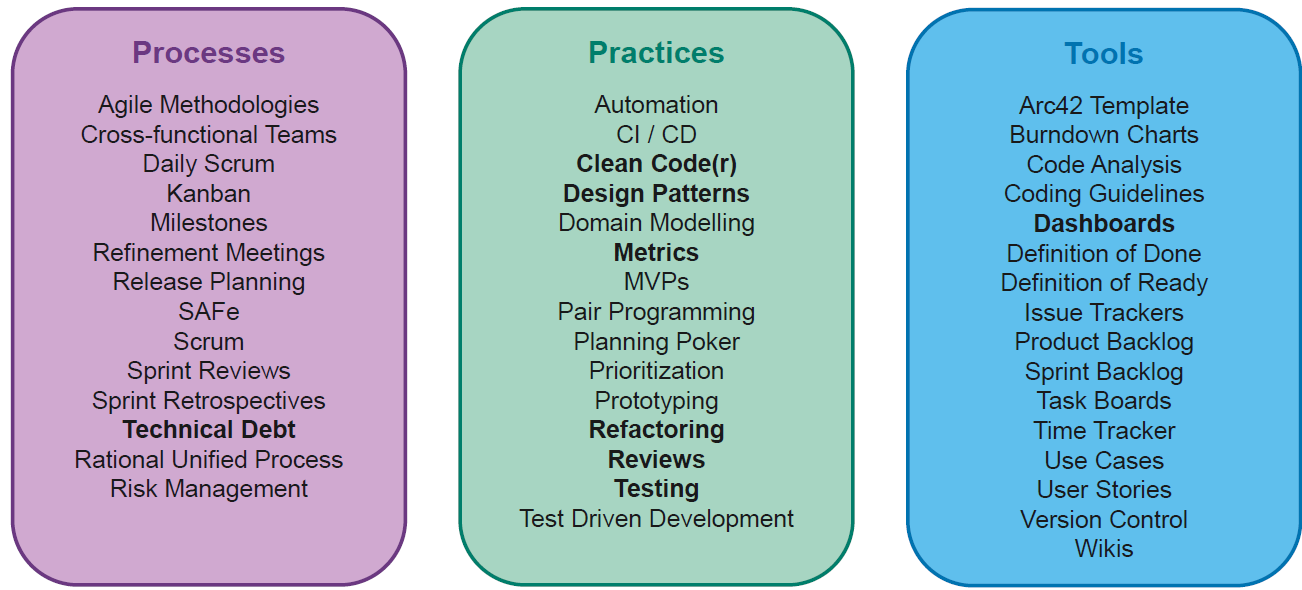
\includegraphics[width=\linewidth]{../img/quality_measures.png}

\subsection{Technical Dept}
\begin{itemize}
    \item Amount of additional rework caused by an easy solution
    \item Not necessary a bad thing
    \item If not repaid, it can grow (interest)
    \item Might not increase linear
\end{itemize}
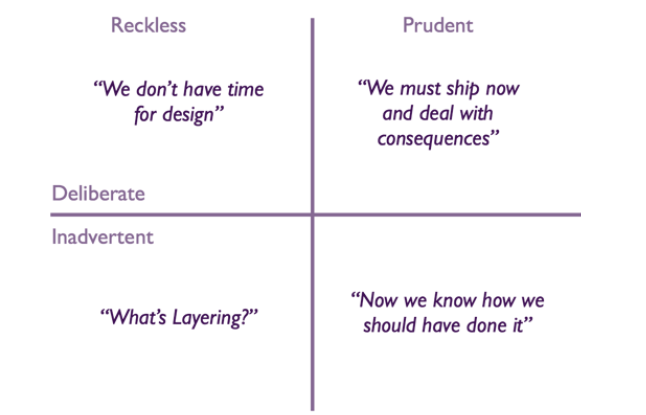
\includegraphics[width=\linewidth]{../img/technical_dept.png}

\subsection{Software Metrics}
\textbf{Product Metrics}
\begin{itemize}
    \item Lines of Code
    \item Code Coverage
    \item Cyclomatic Complexity
\end{itemize}
\textbf{Project Metrics}
\begin{itemize}
    \item Number of Git-Commits
    \item Number of Changed files in Merge-Requests
    \item Number of changes to a file in a time period
\end{itemize}

\subsubsection{Caution}
\begin{itemize}
    \item Only indicators and might be misleading
    \item Acceptable metric does not imply good quality
    \item Choose reasonable scale
    \item Define Actions for unacceptable results
    \item Never use metrics for a reward system
\end{itemize}

\subsubsection{Visualization - Polymetric View}
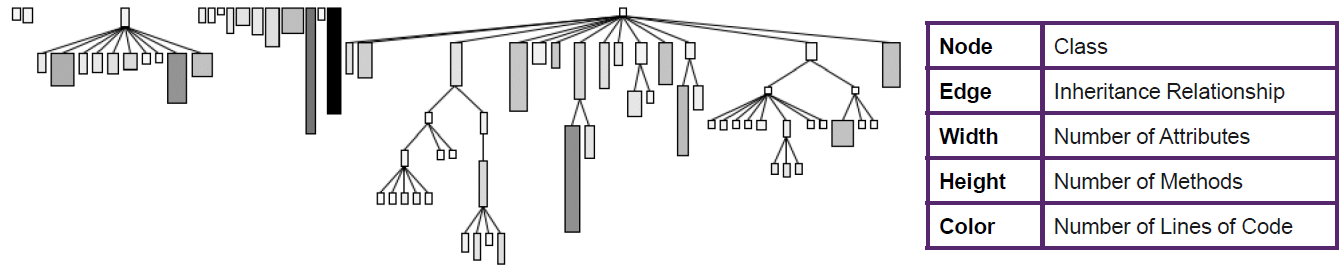
\includegraphics[width=\linewidth]{../img/polymetric_view_1.png}
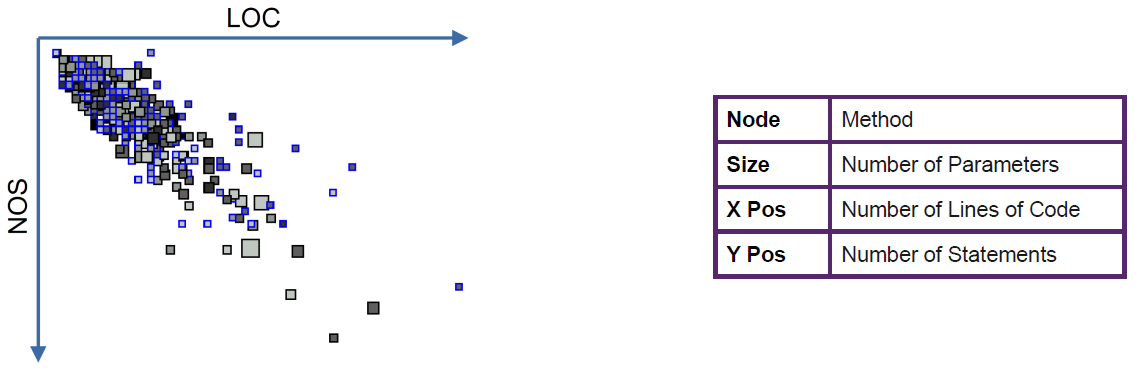
\includegraphics[width=\linewidth]{../img/polymetric_view_2.png}




















        %! Author = Philipp Emmenegger
%! Date = 08/06/2021

\section{Software Architecture}
\textbf{Architecture} focuses on the big picture, the components, boundaries and interfaces.\\
\textbf{Design} addresses smaller challenges within these components\\
\textbf{Inputs for the architecture:}
\begin{itemize}
    \item Functional requirements
    \item Non-functional requirements
    \item Context
    \item Constraints
\end{itemize}

\subsection{Components}
\textbf{Separate by similarity}
\begin{itemize}
    \item Similar in functionality
    \item Similar in technological implementation
\end{itemize}
\textbf{Separate domain from technology}
\begin{itemize}
    \item Domain is stable and long living
    \item Technology is volatile and short living
\end{itemize}

\subsection{Layers vs. Tiers}
\textbf{Layers}
\begin{itemize}
    \item A way of organizing your code
    \item Logical separation by responsibility
\end{itemize}
\textbf{Tiers}
\begin{itemize}
    \item Define where layers are run and deployed
    \item Layers can beb deployed multiple times
\end{itemize}

\subsection{The big three}
\textbf{Adequacy (Angemessenheit)}
\begin{itemize}
    \item Design a system that fits: complexity, team, ...
    \item No Under / Over Engineering
    \item Do not reinvent the wheel
    \item Avoid the golden hammer
\end{itemize}
\textbf{Timeliness}
\begin{itemize}
    \item Eliminate risks early
    \item Decide at the last responsible moment
    \item Do not decite too late
    \item Use time to gather knowledge and experience
\end{itemize}
\textbf{Consistency}
\begin{itemize}
    \item Be consistent within your architecture
    \item Foster consistency using concepts
    \item Use existing concepts when appropriate
\end{itemize}

\subsection{Design}
\textbf{Top-Down}
\begin{itemize}
    \item Provides an overview
    \item Start with the big, work towards the small
    \item Perfect for documentation and communication
\end{itemize}
\textbf{Bottom-Up}
\begin{itemize}
    \item Addresses technical risks
    \item Solve a single problem, generalize afterwards
    \item Might lead to insufficient consistency
\end{itemize}

\subsection{Anti-Patterns}
\begin{itemize}
    \item Over Engineering
    \item Under Engineering
    \item Gold Hammer
    \item Reinvent the wheel
    \item Design in an ivory tower
    \item Design by power point
    \item Design by market
    \item Design for resume
\end{itemize}

\subsection{Documentation}
\begin{itemize}
    \item Correctness
    \item Maintainability
    \begin{itemize}
        \item use templates and standarts
    \end{itemize}
    \item Understandability
    \item Adequateness
\end{itemize}

\subsubsection{arc42 template}
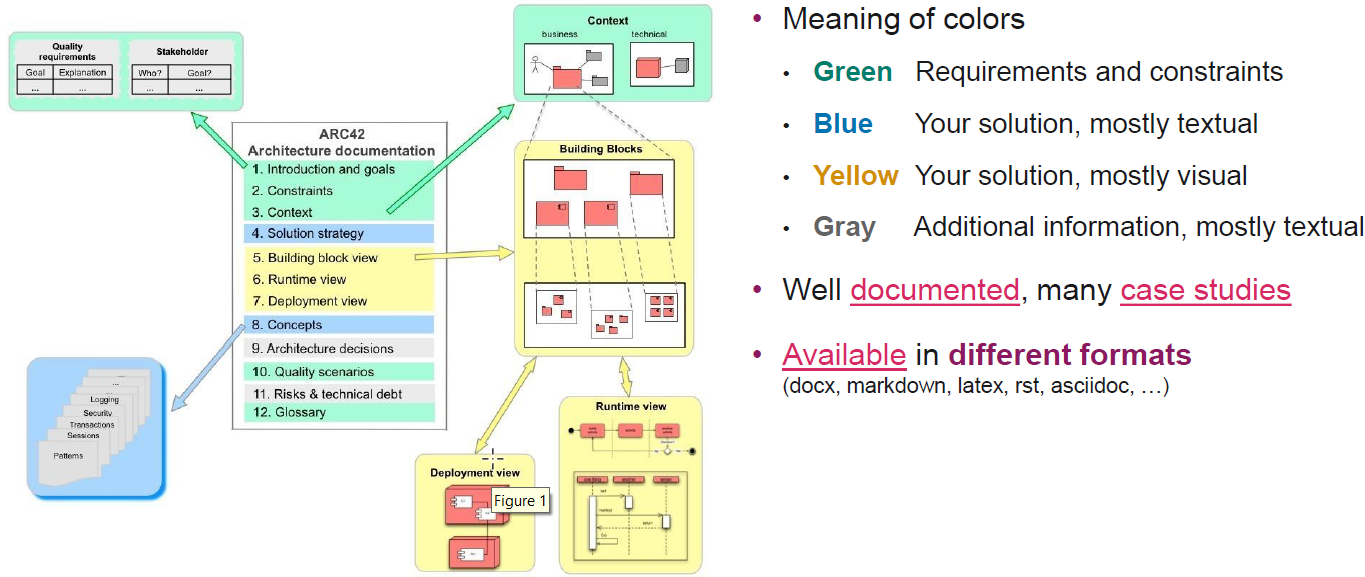
\includegraphics[width=\linewidth]{../img/arc42.png}

\subsection{Patterns}
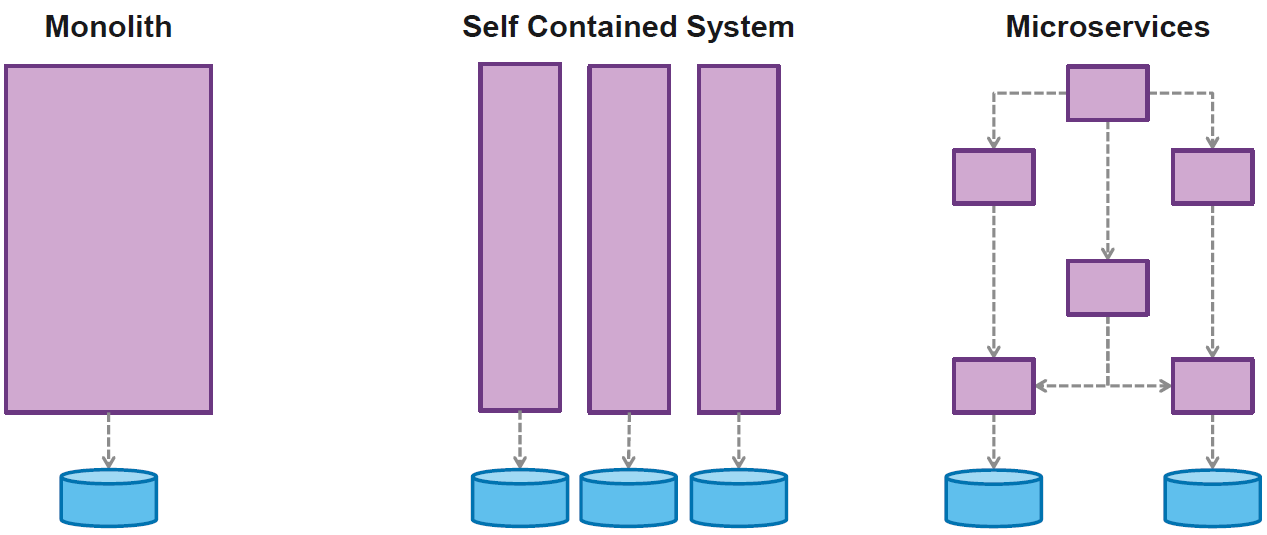
\includegraphics[width=\linewidth]{../img/architecture_patterns_1.png}
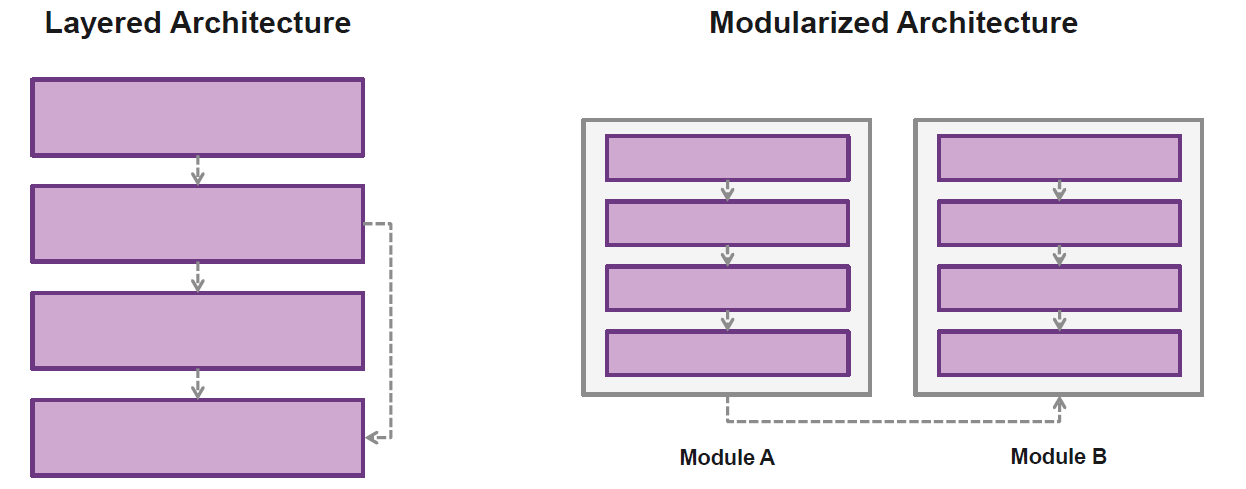
\includegraphics[width=\linewidth]{../img/architecture_patterns_2.png}
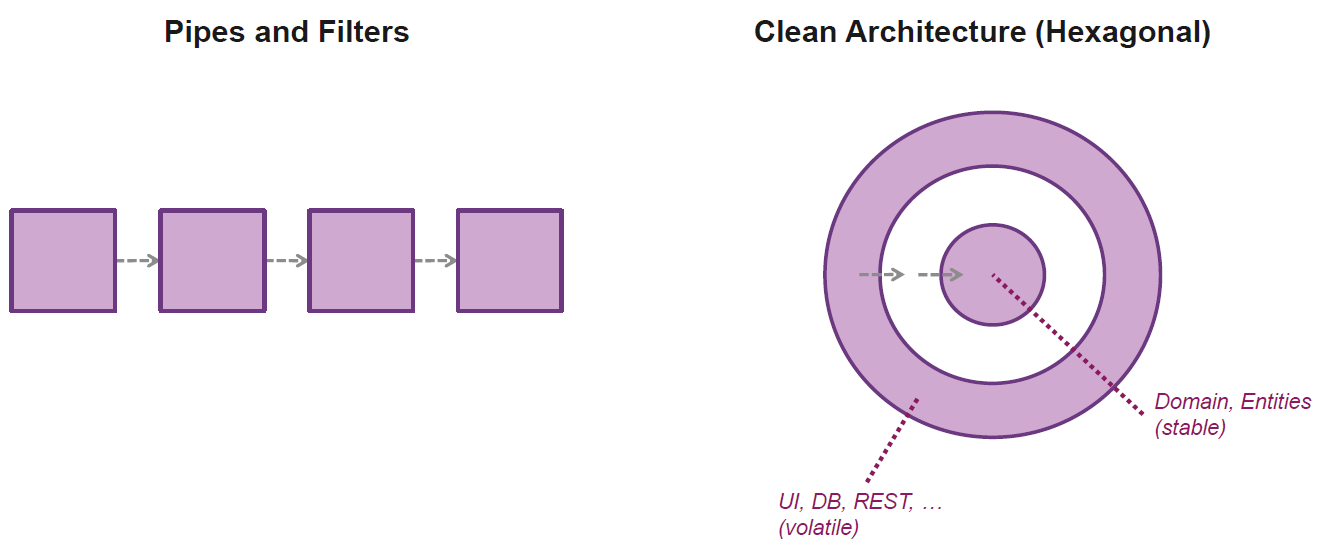
\includegraphics[width=\linewidth]{../img/architecture_patterns_3.png}












        %! Author = Philipp Emmenegger
%! Date = 08/06/2021

\section{Clean Code}
\subsection{Fundamentals}
\subsubsection{YAGNI}
\textbf{YAGNI - You Aren't Gonna Need It}
\begin{itemize}
    \item Code, that has never been written, can not rot
    \item Less code means less complexity
    \item Agile Mindset
\end{itemize}

\subsubsection{KISS}
\textbf{KISS - Keep it simple, stupid!}
\begin{itemize}
    \item Simple code tends to be more readable
    \item If there are options - choose the simple one
    \item Beware of premature optimizations
\end{itemize}

\subsubsection{Names}
\textbf{Positive Characteristics}
\begin{itemize}
    \item Intention-revealing
    \item Pronounceable
    \item Searchable
    \item Length matches scope
    \item Classes named with nouns
    \item Methods start with verb
    \item Consistent
    \item Domain-terminology
\end{itemize}
\textbf{Things to avoid}
\begin{itemize}
    \item Disinformation
    \item Similarity
    \item Encoding
    \item Magic numbers
\end{itemize}

\subsubsection{Functions}
\textbf{Positive Characteristics}
\begin{itemize}
    \item Short
    \item Ascertainable (line length < screen width)
    \item Short parameter lists
    \item Name starts with verb
    \item Name reflects responsibility
    \item Single responsibility
    \item One level of abstraction
    \item Command or query
\end{itemize}
\textbf{Things to avoid}
\begin{itemize}
    \item Duplication (DRY)
    \item Indent level > 2
    \item Side effects
    \item Output arguments
    \item Return codes
    \item Inappropriate use of switch
    \item Inappropriate use of try .. catch
\end{itemize}

\subsubsection{Classes}
\textbf{Positive Characteristics}
\begin{itemize}
    \item Short > 200 lines
    \item Straightforward signature
    \item Named with a noun
    \item Name reflects responsibility
    \item Hiding information
    \item High cohesion
    \item Single responsibility (SRP, ISP)
    \item Open for extension
    \item Isolated from change (DIP)
\end{itemize}
\textbf{Things to avoid}
\begin{itemize}
    \item Tight coupling
    \item Talking to strangers
    \item God classes
    \item Manager classes
\end{itemize}

\textbf{Cohesion} is the degree to which the elements inside a class belong together.\\
High cohesion often correlates with loose coupling and vice verca:
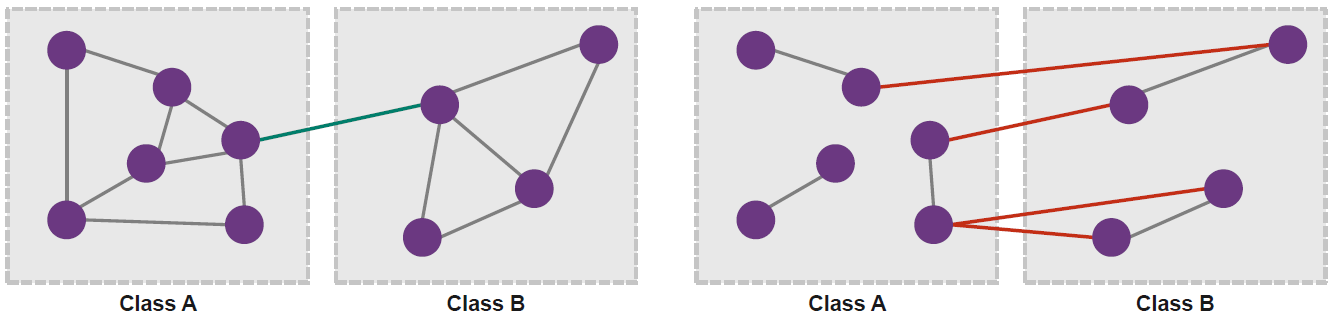
\includegraphics[width=\linewidth]{../img/cohesion.png}

\subsubsection{Classes - Law of Demeter}
\begin{itemize}
    \item Classes should not know the details of the objects it manipulates
    \item Don't talk to strangers!
    \item Tell, don't lie!
\end{itemize}
\begin{lstlisting}
car.getEngine().start();    // bad
car.prepareForRide();       // good
\end{lstlisting}

\subsubsection{Error Handling}
\begin{itemize}
    \item Use exceptions instead of error codes
    \item Add a precise description of the error
    \item Avoid returning null
\end{itemize}

\subsubsection{Comments}
\begin{itemize}
    \item Indicates bad code
    \item Instead of a comment, improve your code
    \item Very hard to maintain
    \item Can be misleading when outdated
    \item Add noise to the code
\end{itemize}
\textbf{Appropriate uses of comments:}
\begin{itemize}
    \item Explanation or information
    \item Warning of consequences
    \item Legal comments
    \item Highlight work in progress
\end{itemize}
\textbf{Things to avoid}
\begin{itemize}
    \item Redundant comments
    \item Extensive comments
    \item Misleading comments
    \item Mandated comments
    \item Jounal comments
    \item Position markers / seperators
    \item commented-out code
\end{itemize}

\subsection{Design Principles}
\subsubsection{DRY - Don't Repeat Yourself}
\begin{itemize}
    \item Duplication: primary enemy of maintainability
    \item Bugs must be fixed multiple times
    \item Features must be added multiple times
    \item Forget any copy and the nightmare begins
\end{itemize}

\subsubsection{OLA - One Level of Abstraction}
\begin{itemize}
    \item Keeping one level of abstraction fosters readability
    \item aka. Single Level of Abstraction
\end{itemize}
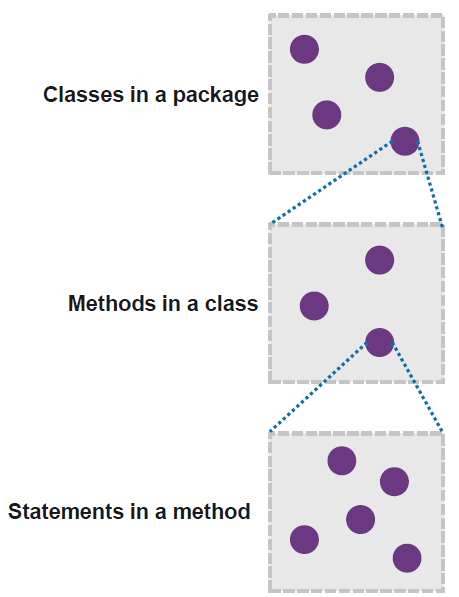
\includegraphics[width=0.5\linewidth]{../img/OLA.png}

\subsubsection{SRP - Single-Responsibility Principle}
\begin{itemize}
    \item A class, module or functio should have only one single reason to change
    \item Compose software of many small classes
\end{itemize}

\subsubsection{OCP - Open-Closed Principle}
\begin{itemize}
    \item Software entities should be open for extension but closed for modification
    \item Possible to add functionality without changing existing code
    \item Inheritance / Composition
\end{itemize}

\subsubsection{LSP - Liskov Substitution Principle}
\begin{itemize}
    \item Subtypes must behave like their base type
    \item A subtype may extend base type functionality but must not reduce it
\end{itemize}

\subsubsection{ISP - Interface Segregation Principle}
\begin{itemize}
    \item A client shall only depend on the details which it does use
    \item Extracting interfaces / super classes
    \item The leaner the service interface is, the smaller the coupling of both components
    \item Increased readability
\end{itemize}

\subsubsection{DIP - Dependency Inversion Principle}
\begin{itemize}
    \item High-level classes must not depend on low-level classes
    \item Low-level classes can be replaced
    \item Dependency Injection
\end{itemize}

\subsubsection{CQS - Command Query Separation}
\begin{itemize}
    \item Every method should either perform an action or a query that returns data
    \item Querying methods are side-effect free
\end{itemize}












        %! Author = Philipp Emmenegger
%! Date = 09/06/2021

\section{Clean Coder}
\subsection{Values}
\textbf{Professionalism}
\begin{itemize}
    \item Take responsibility for your work
    \begin{itemize}
        \item Do no harm to function
        \item Do no harm to structure
        \item Do know that your solution works
        \item Do know that your solution is well designed
    \end{itemize}
    \item Have appropriate work ethic
    \begin{itemize}
        \item Know your field - but keep learning
        \item Practice, also outside your normal job
        \item Collaborate and communicate with your team
        \item Regularly reflect your attitude and behaviour
    \end{itemize}
    \item Be pragmatic
\end{itemize}

\subsection{Attitudes}
\textbf{Saying no}
\begin{itemize}
    \item Say no when you think its the right thing to do
    \item Explain the reason, offer alternatives
    \item There is no trying - if you are unsure, say no
\end{itemize}
\textbf{Saying yes}
\begin{itemize}
    \item If you mean it and can handle the task
    \item Work hard to keep your promises
\end{itemize}
\textbf{Coding}
\begin{itemize}
    \item Be physically and psychically prepared for coding
    \item Pace yourself
    \item Regular breaks
    \item Prepare for interruptions
    \item Get help if you're stuck
    \item Programm deliberately
\end{itemize}
\textbf{Time Management}
\begin{itemize}
    \item Recharge before important work
    \item Meetings
    \begin{itemize}
        \item Necessary
        \item Huge time waster
        \item Only attend meetings that seem valuable
    \end{itemize}
\end{itemize}
\textbf{Practicing}
\begin{itemize}
    \item Keep your knowledge up to date
\end{itemize}

\subsection{Techniques}
\textbf{Time Boxing}
\begin{itemize}
    \item Seperate your day in focus and non-focus time slots
    \item Pomodoro Technique
    \item Nothing interferes with your 25min of focus time
    \item Address all interruptions in the break or next slot
\end{itemize}
\textbf{Coding Katas}
\begin{itemize}
    \item Make the movements automatic and instinctive
    \item Practice skills in safe situations
    \item Bowling, Tennis, Poker Hands, Gilded Rose, ...
\end{itemize}
\textbf{Coding Dojos}
\begin{itemize}
    \item A place to practice programming
    \item Learn from each other
    \item \textit{Wasa} - Train as pair of two devs
    \item \textit{Randori} - Trans as a group of devs
    \begin{enumerate}
        \item Dev 1: write a failing test
        \item Dev 2: make test pass, write failing test
        \item repeat...
    \end{enumerate}
\end{itemize}
\textbf{Pair Programming}
\begin{itemize}
    \item Driver: writes code, focus on current task
    \item Navigator: gives constant feedback, focus on big picture
    \item switch roles frequently
    \item Benefits
    \begin{itemize}
        \item Fewer defects in code
        \item Better SW design
        \item Interrupts can be handled easy
        \item Knowledge transfer
        \item Team building
    \end{itemize}
    \item Drawbacks
    \begin{itemize}
        \item More time consumption
    \end{itemize}
\end{itemize}
\textbf{Rubber Duck Debugging}
\begin{itemize}
    \item You can not find the root of a problem
    \item Explain it to someone else - change perspective
    \item Requires deep understanding
    \item Someone - can be rubber duck
\end{itemize}

























        %! Author = Philipp Emmenegger
%! Date = 09/06/2021

\section{Design Patterns}
\begin{itemize}
    \item Stories of repeatedly successful engineering
    \item Explaining the context and/or problem
    \item Describing a generic solution
    \item Mentoring viable alternatives
    \item Listing benefits and drawbacks
\end{itemize}
\textit{Design patterns are...}
\begin{itemize}
    \item Discoveries not inventions
    \item an efficient vocabulary
    \item describing a generic solution with "roles"
    \item honest
\end{itemize}
\textit{Are not...}
\begin{itemize}
    \item ready to use
    \item a golden hammer for every problem
    \item replacements for design principles
    \item replacements for software architecture
\end{itemize}

\subsection{Patterns vs. Principles}
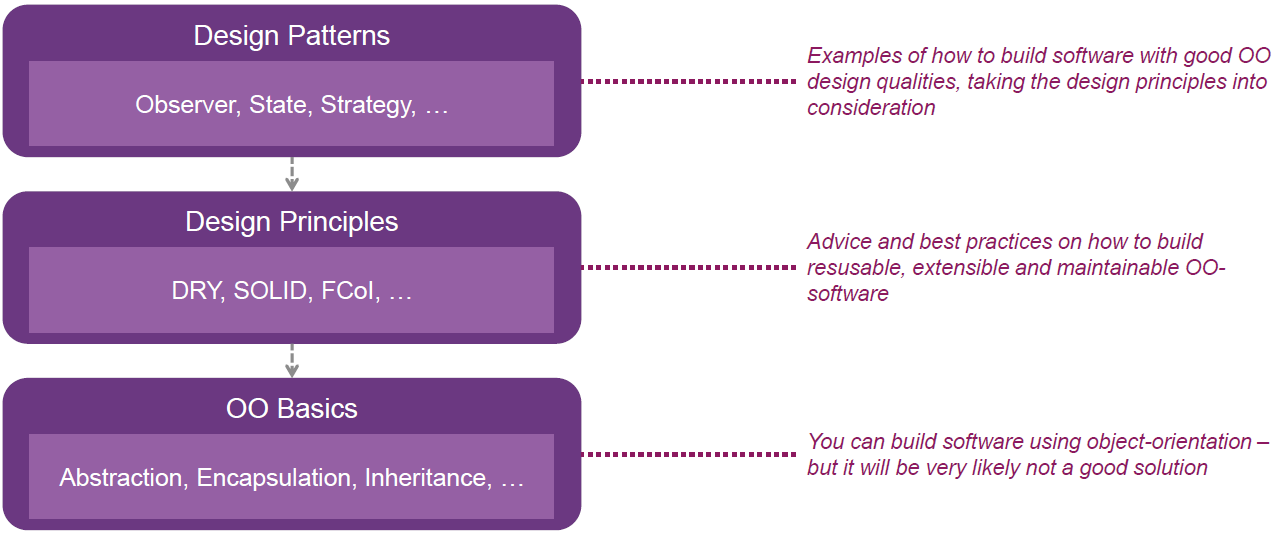
\includegraphics[width=\linewidth]{../img/patterns_vs_principles.png}

\subsection{GoF Design patterns}
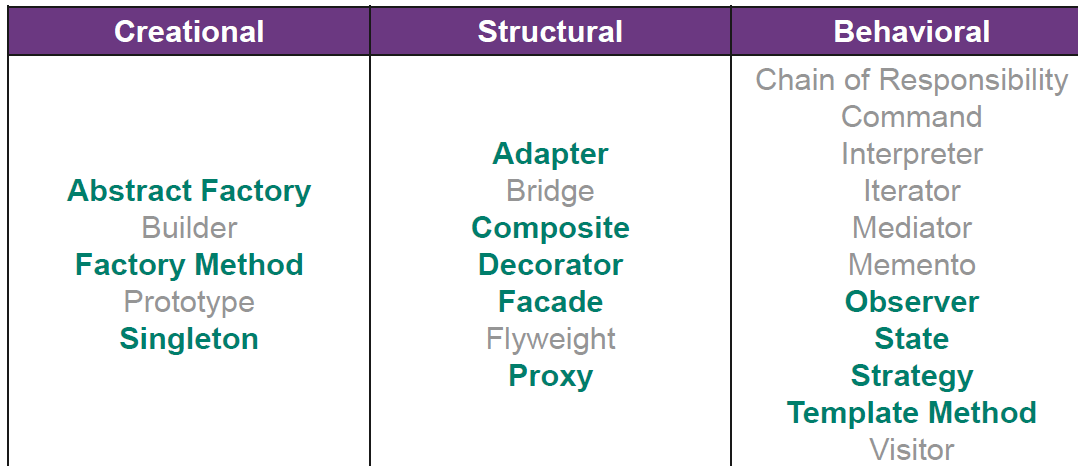
\includegraphics[width=\linewidth]{../img/gof_design_patterns.png}

\subsection{MVC, MVP, MVVM}
\begin{itemize}
    \item Design patterns dealing with presentation
    \item Not from the GoF book
    \item Very often compound from GoF-patterns
    \begin{itemize}
        \item Composite: to build a control-hierarchy
        \item Observer: to inform V about changes
        \item Strategy: to decouple V from C/P
    \end{itemize}
\end{itemize}

\subsection{Observer}
Define a one-to-many dependency between objects so that when one object changes state, all its dependents are notified and updated automatically.\\
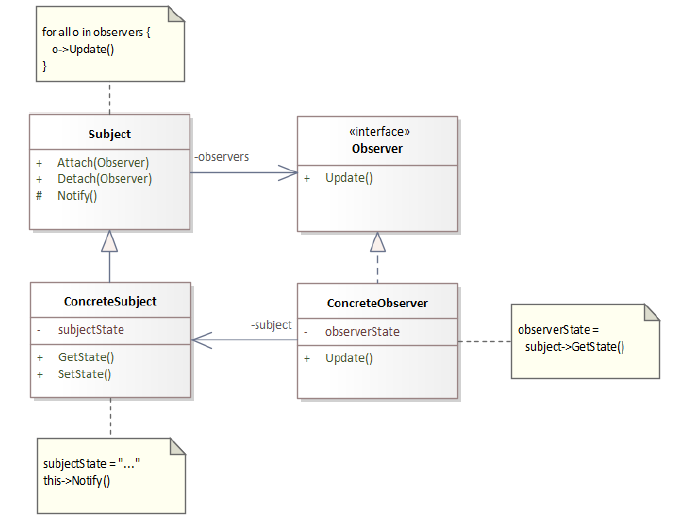
\includegraphics[width=0.85\linewidth]{../img/observer_pattern.png}

\subsection{State}
Allow an object to alter its behaviour when its internal state changes. The object will appear to change its class.
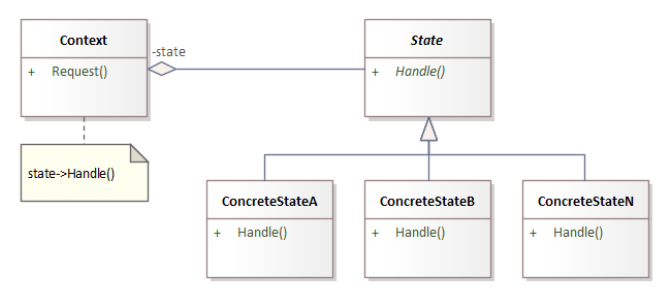
\includegraphics[width=0.85\linewidth]{../img/state_pattern.png}
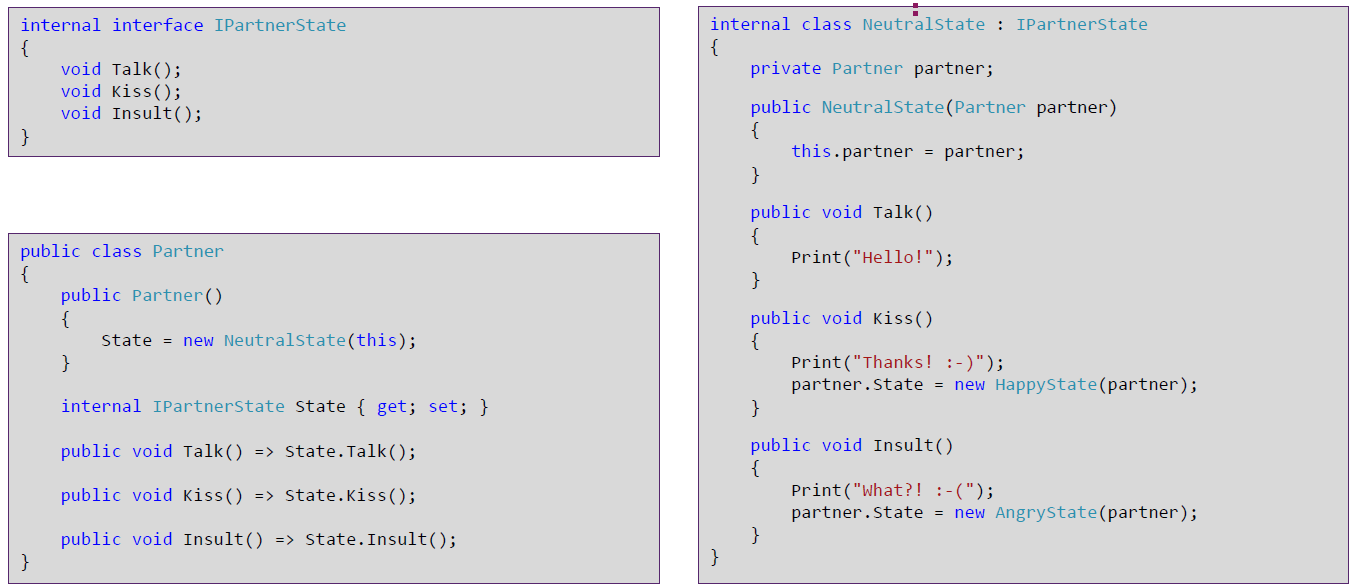
\includegraphics[width=\linewidth]{../img/state_pattern_code.png}

\subsection{Strategy}
Define a family of algorithms, encapsulate each one and make them interchangeable.\\
Strategy lets the algorithm vary independently from clients that use it.\\
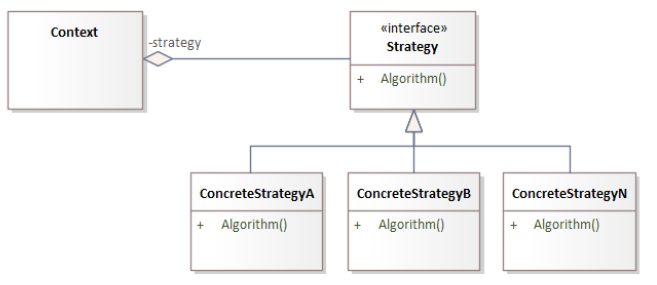
\includegraphics[width=0.85\linewidth]{../img/strategy_pattern.png}
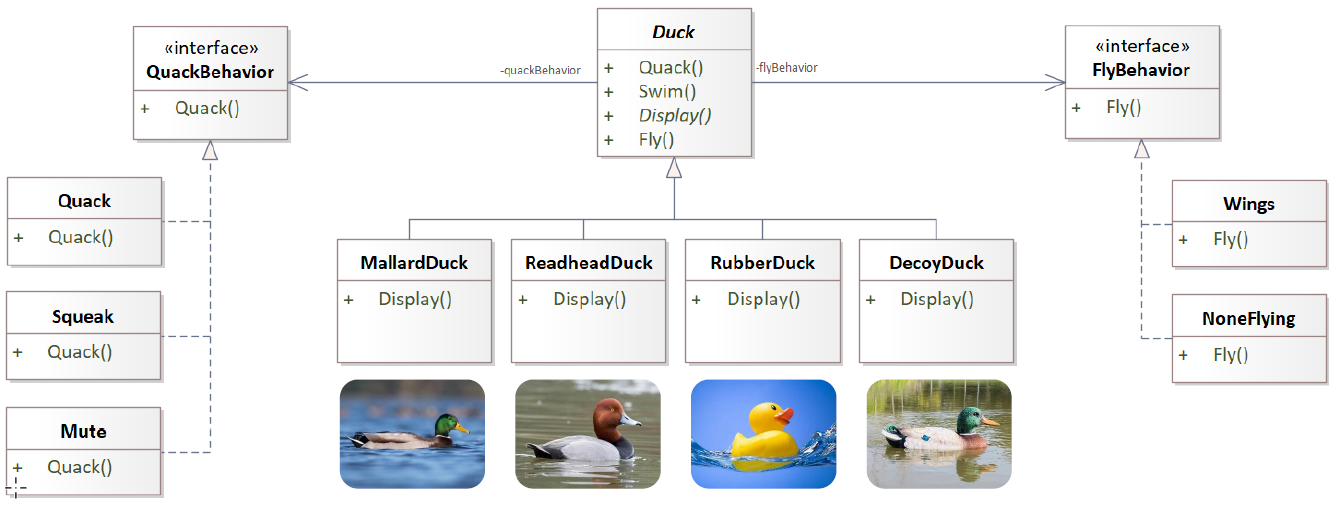
\includegraphics[width=\linewidth]{../img/strategy_pattern_duck_pond.png}
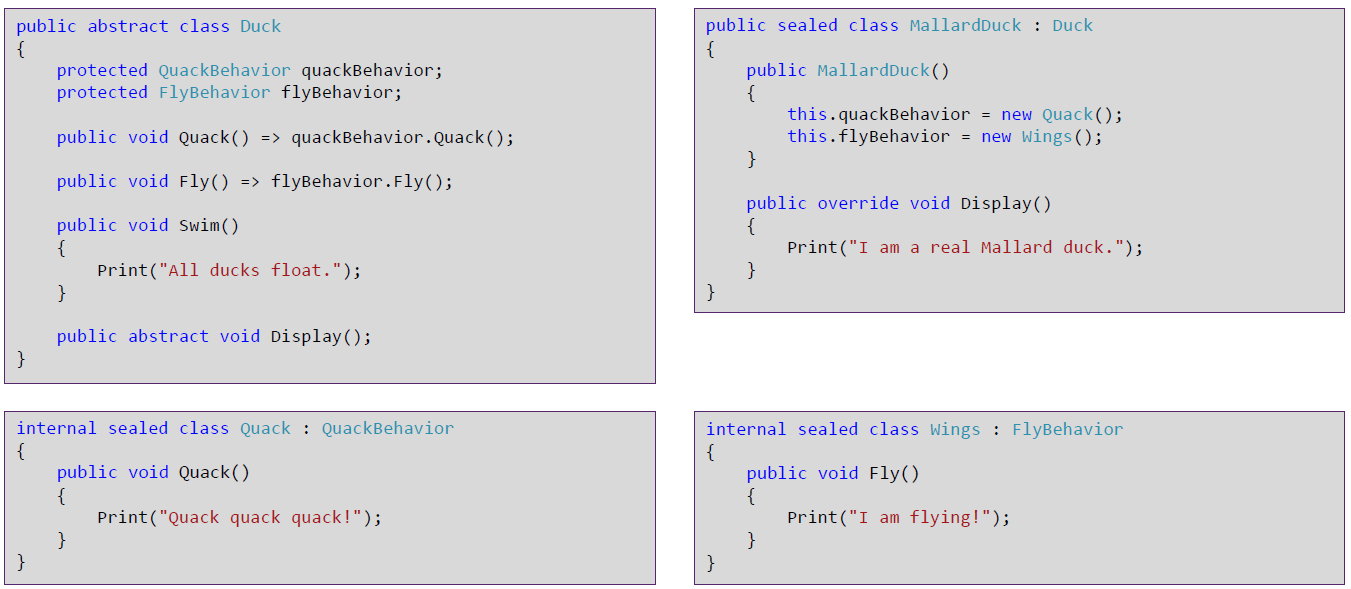
\includegraphics[width=\linewidth]{../img/strategy_pattern_code.png}

\subsubsection{NULL-Objects}
\begin{itemize}
    \item Classes implementing an interface wih empty methods
    \item Mute / NoneFlying in Duck Game
    \item Useful to get rid of null-checks and the risk of NullPointerException
\end{itemize}

\subsubsection{Dependency Injection}
\begin{itemize}
    \item Possible to get rid of all subtypes and inject the full behaviour using the constructor
    \item Constructor injection
\end{itemize}
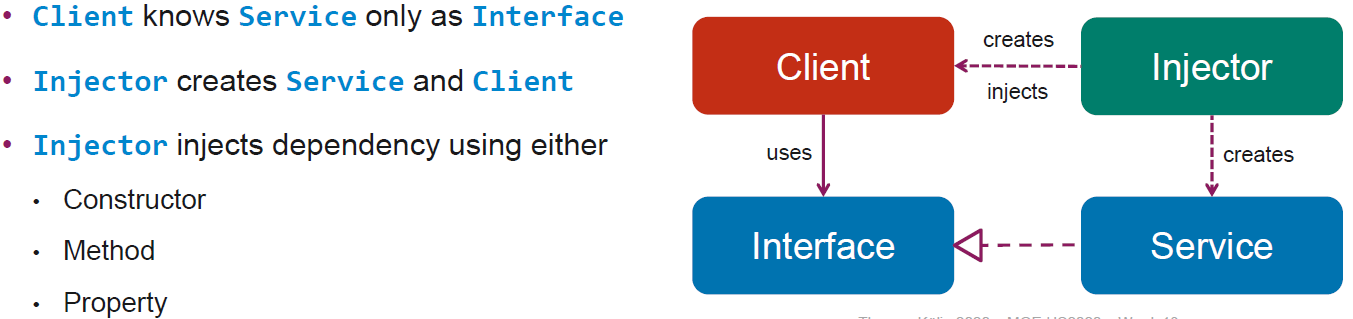
\includegraphics[width=\linewidth]{../img/strategy_pattern_DI.png}

\subsection{Strategy vs. State}
\textbf{State Pattern}
\begin{itemize}
    \item Encapsulates state behaviour
    \item Context hides internal state transitions
    \item Context switches its visible behaviour
    \item Replaces conditionals with compositions
\end{itemize}
\textbf{Strategy Pattern}
\begin{itemize}
    \item Encapsulates algorithmic behaviour
    \item Clients can configure Context with strategy
    \item Context mostly remains its visible behaviour
    \item Replaces inheritance with composition
\end{itemize}

\subsection{Template Method}
Define the skeleton of an algorithm in an operation, deferring some steps to subclasses.\\
Template Method lets subclasses redefine certain steps of an algorithm without changing the algorithm's structure.\\
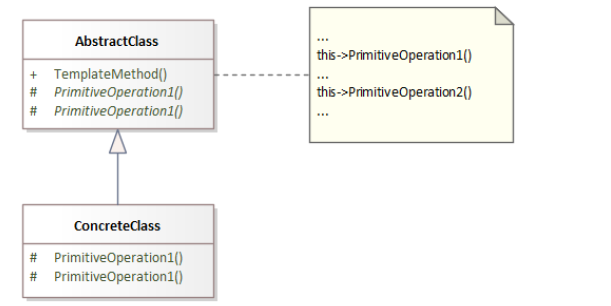
\includegraphics[width=0.7\linewidth]{../img/template_method.png}\\
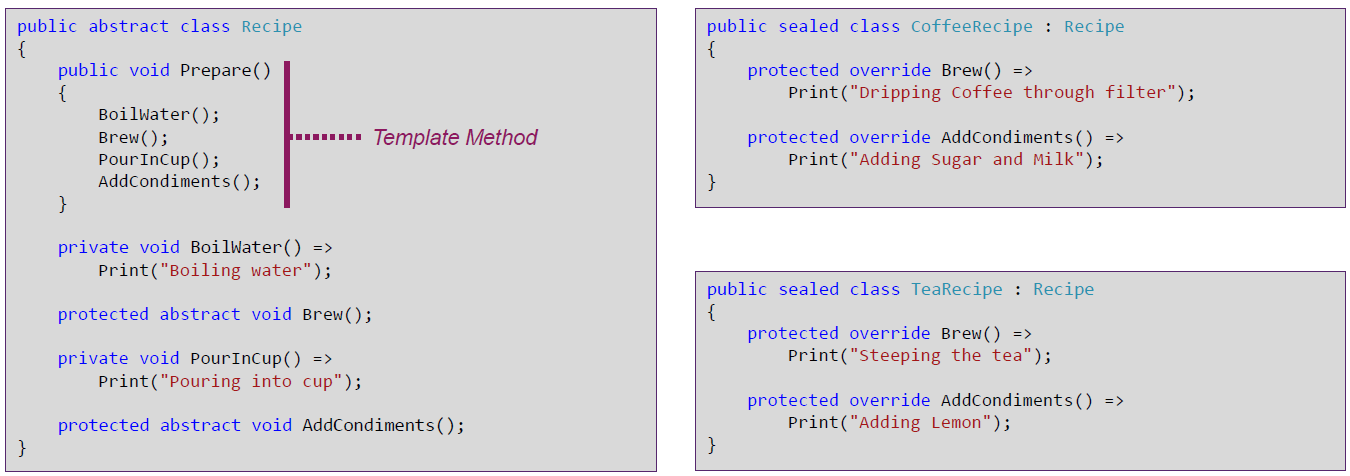
\includegraphics[width=\linewidth]{../img/template_method_code.png}




























        %! Author = Philipp Emmenegger
%! Date = 09/06/2021

\subsection{Factory Method}
Define an interface for creating an object, but let subclasses decide which class to instantiate.\\
Factory Method lets a class defer instantiation to subclasses.\\
\begin{itemize}
    \item Can be \textit{abstract} or \textit{virtual}
    \item Can be parameterized
    \item Typically called from within a Template Method
    \item Names start with \textit{Create}-prefix
\end{itemize}

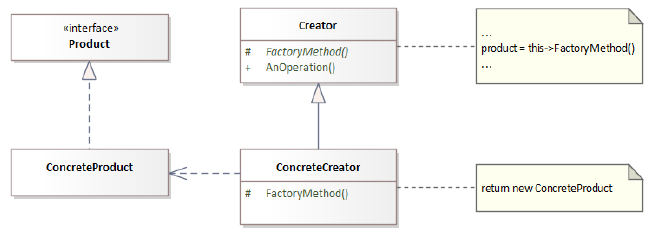
\includegraphics[width=\linewidth]{../img/factory_method.png}
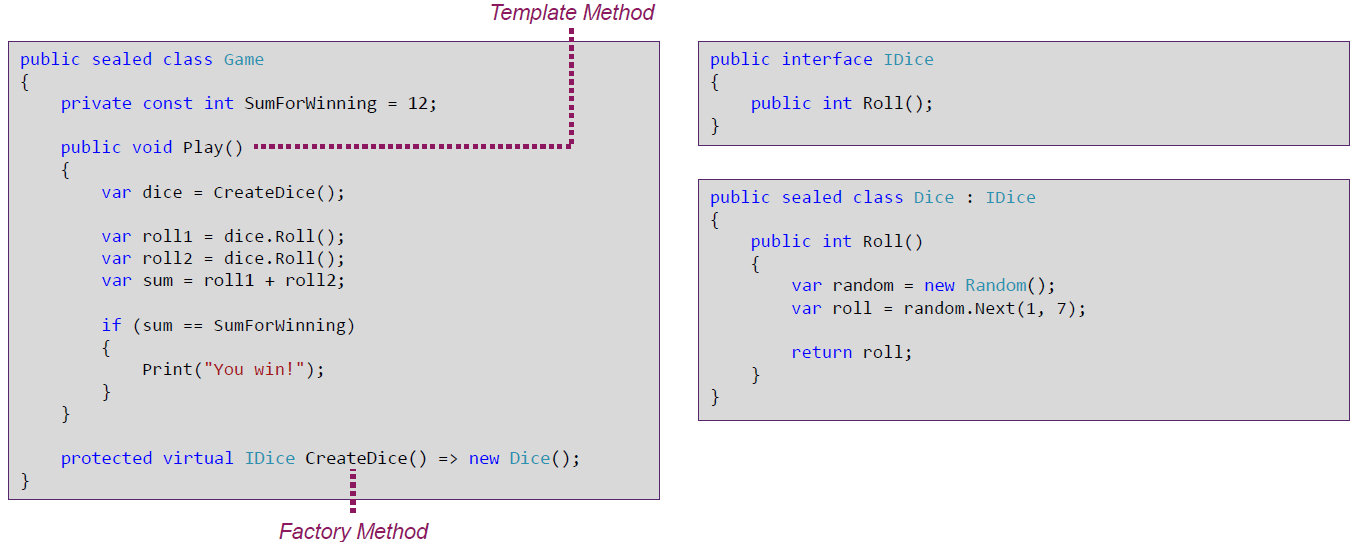
\includegraphics[width=\linewidth]{../img/factory_method_code.png}

\subsection{Abstract Factory}
Provide an interface for creating families of related or dependent objects without specifying their concrete classes.\\
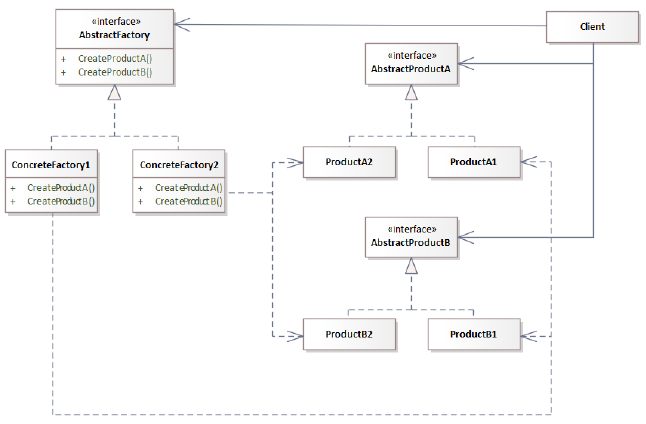
\includegraphics[width=\linewidth]{../img/abstract_factory.png}
\begin{itemize}
    \item Composition should be favored over inheritance
    \item Object creation is a responsibility - can justify a seperate class (SRP)
    \item Move object creation to a class called Factory
    \item Inject an object of that factory into the Game
\end{itemize}
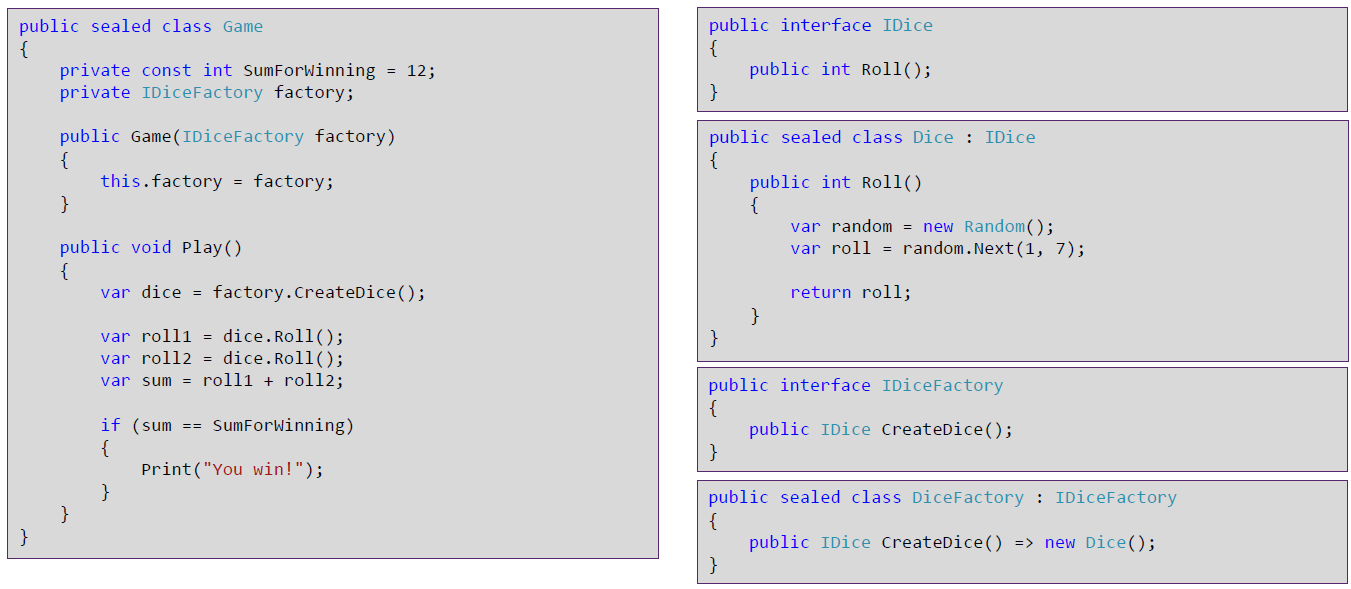
\includegraphics[width=\linewidth]{../img/abstract_factory_code.pong.png}

\subsection{(Simple) Factory}
\begin{itemize}
    \item Strategy for creating objects
    \item Creating objects with hardcoded values
    \item Creating objects read from a database
    \item Creating objects read from a webservice
\end{itemize}
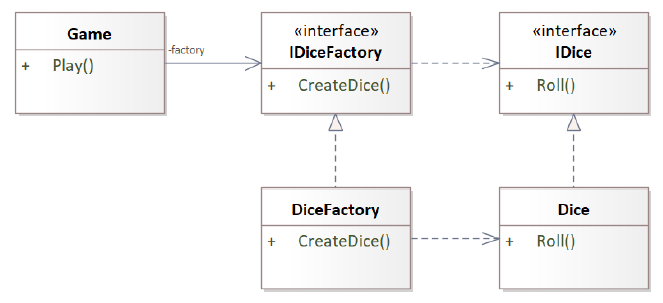
\includegraphics[width=0.7\linewidth]{../img/factory_pattern.png}

\subsection{Singleton}
Ensure a class only has one instance, and provice a global point of access to it.\\
\textbf{Drawbacks:}
\begin{itemize}
    \item Globals with high coupling
    \item Hard to test
    \item Error-prone when multi-threading
\end{itemize}
\textbf{If you need a single instance:}
\begin{itemize}
    \item Create it in your main and inject it
    \item Let a Factory or Proxy manage its lifecycle
\end{itemize}
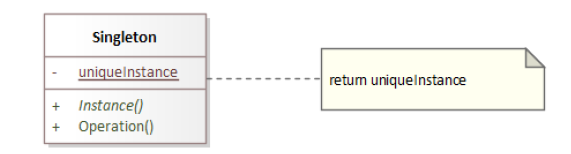
\includegraphics[width=0.7\linewidth]{../img/singleton_pattern.png}\\
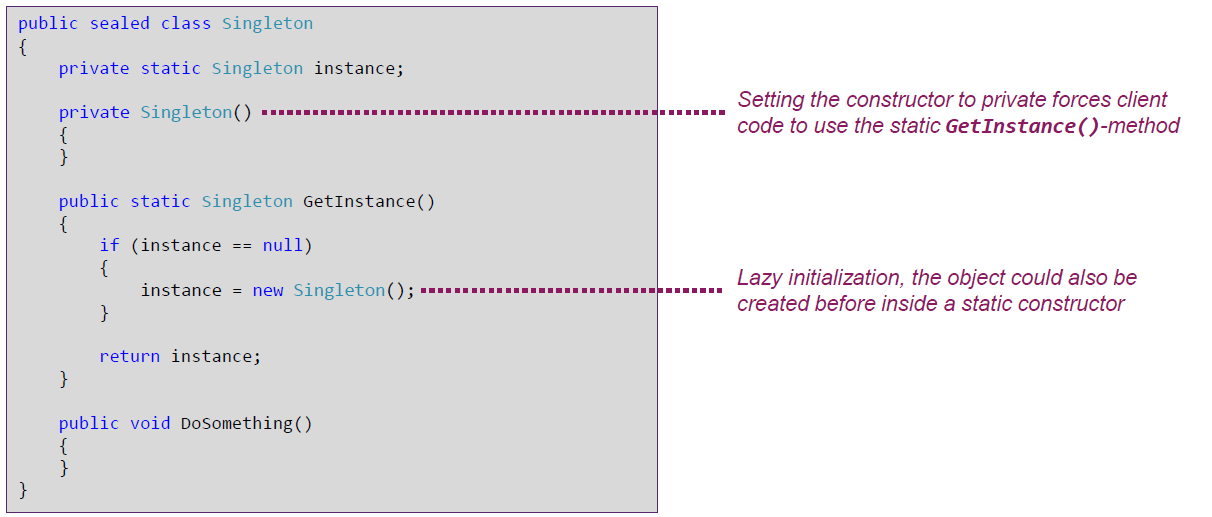
\includegraphics[width=\linewidth]{../img/singleton_pattern_code.png}

\subsection{Adaper}
Convert the interface of a class into another interface clients expect.\\
Adapter lets classes work together that couldn't otherwise because of incompatible interfaces.\\
\begin{itemize}
    \item Adapter can add functionality to Adaptee
    \item If creating the Adaptee is complex, think about Injection or Factories
\end{itemize}
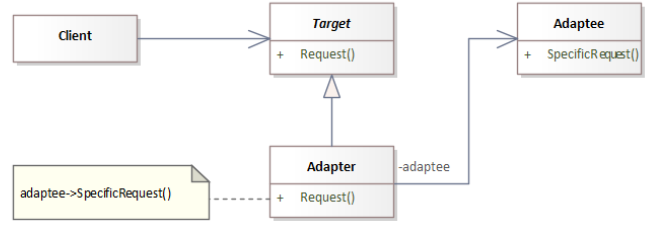
\includegraphics[width=0.7\linewidth]{../img/adapter_pattern.png}\\
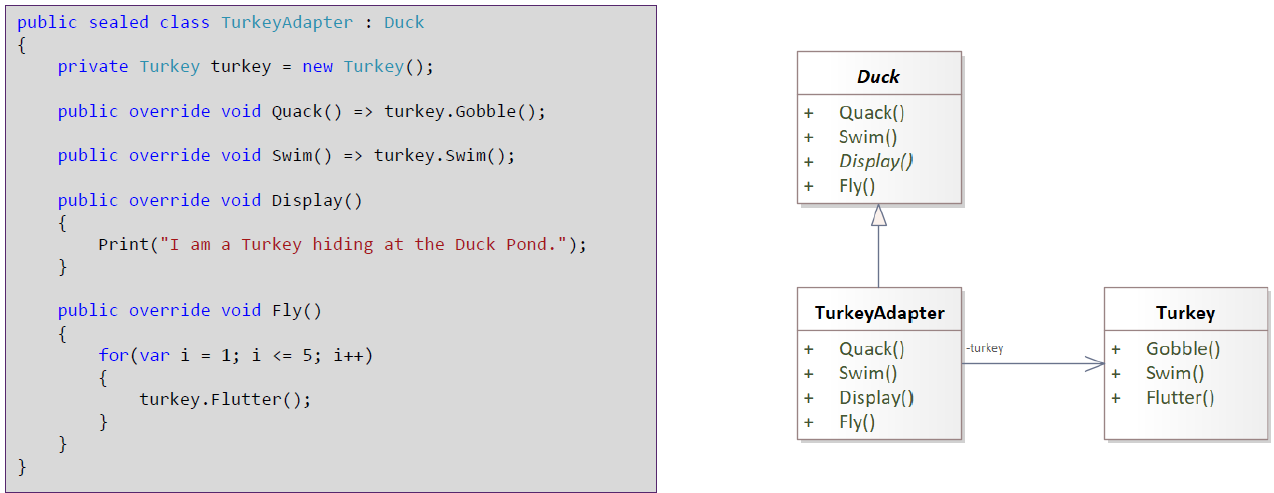
\includegraphics[width=\linewidth]{../img/adapter_pattern_code.png}\\
\subsubsection{Variants}
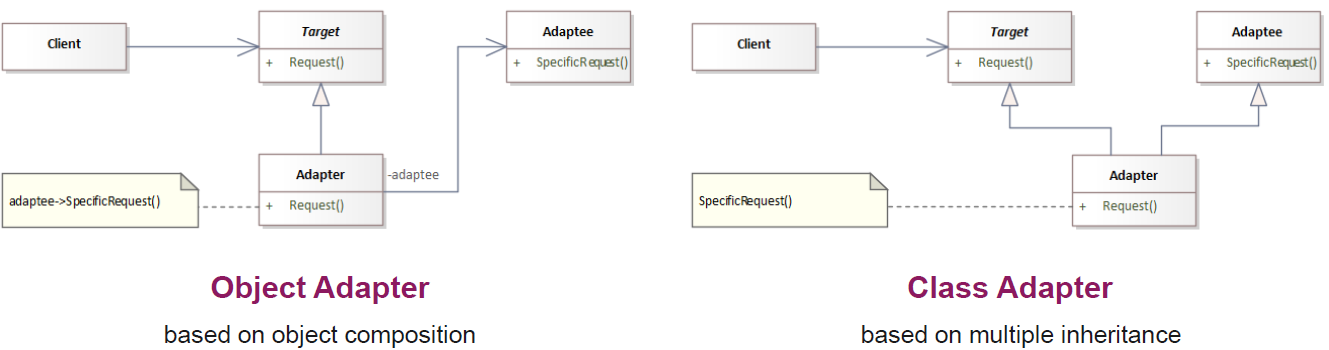
\includegraphics[width=\linewidth]{../img/adapter_pattern_variants.png}

\subsection{Facade}
Provide a unified interface to a set of interfaces in a subsystem.\\
Facade defines a higher-level interface that makes the subsystem easier to use.\\
\begin{itemize}
    \item Decouples a client from a complex, internal / external subsystem
    \item Keep the interface of the Facade small
    \item Multiple Facades for the same subsystem possible (SRP)
    \item Helps to achieve exchangeability
\end{itemize}
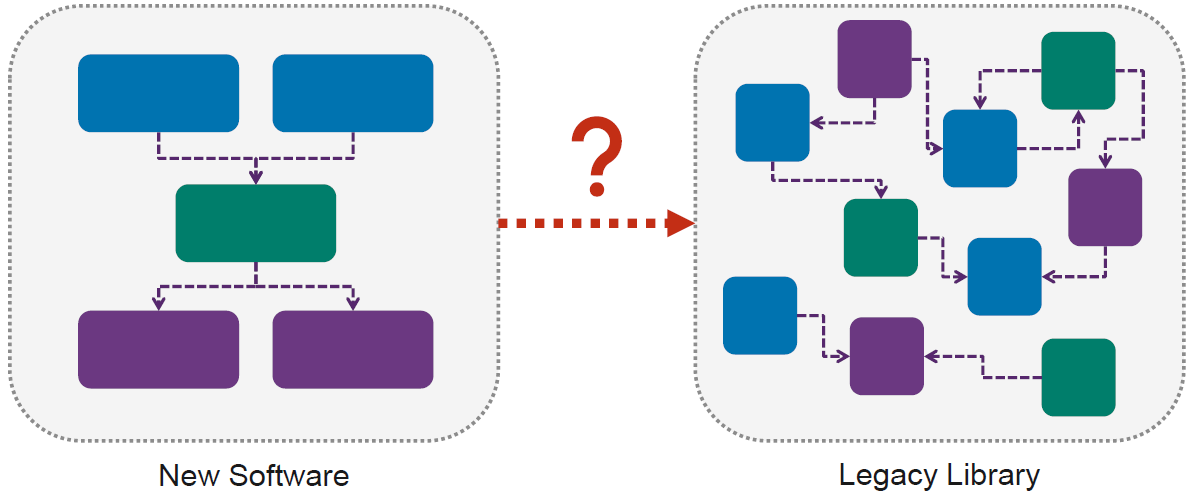
\includegraphics[width=\linewidth]{../img/facade_pattern.png}

\subsection{Composite}
Compose objects into tree structures to represent part-whole hierarchies.\\
Conposite lets clients treat individual objects and compositions of objects uniformly.\\
\begin{itemize}
    \item Trade off between SRP and transparency
    \item Component as interface / abstract class possible
    \item Component with abstract or virtual methods possible
\end{itemize}
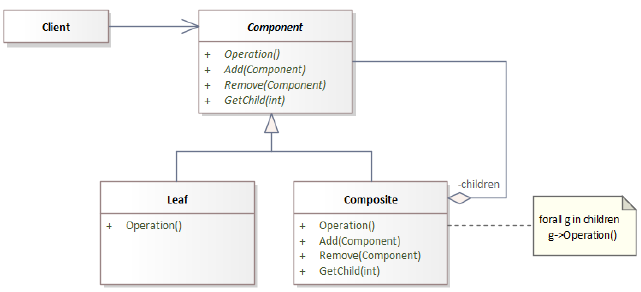
\includegraphics[width=0.7\linewidth]{../img/composite_pattern.png}\\
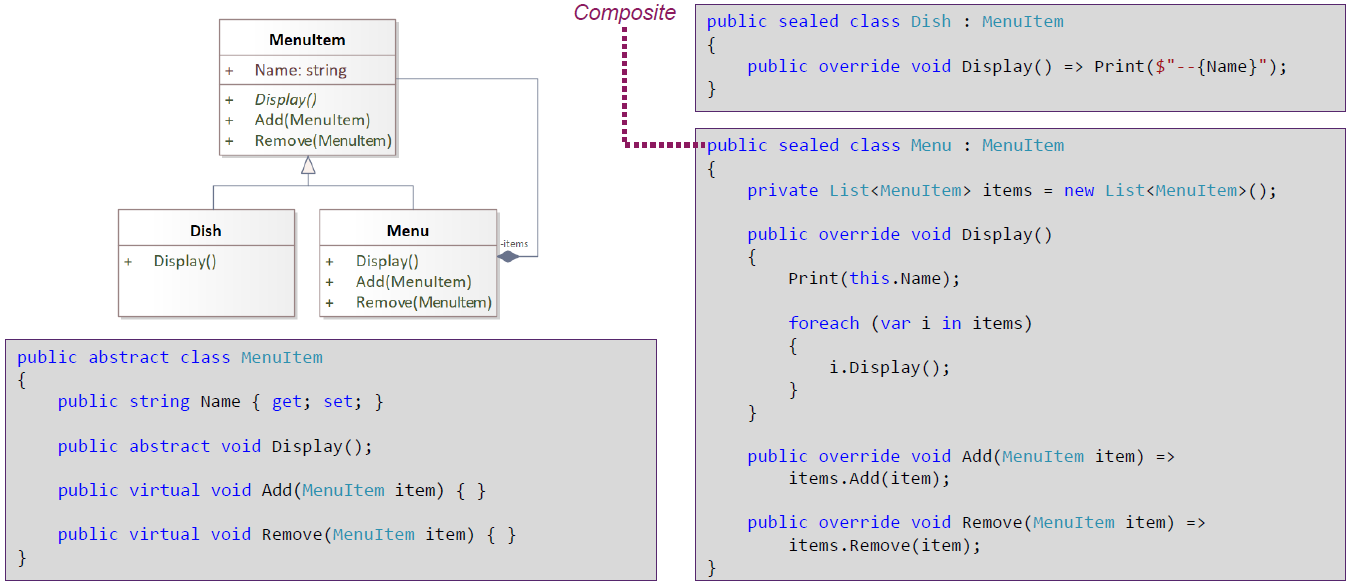
\includegraphics[width=\linewidth]{../img/composite_pattern_code.png}\\
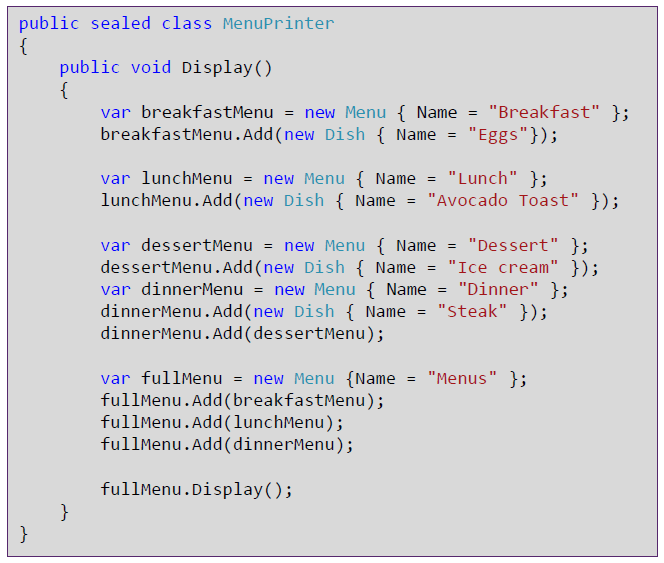
\includegraphics[width=0.7\linewidth]{../img/composite_pattern_code_2.png}\\

\subsection{Decorator}
Attach additional responsibilites to an object dynamically.\\
Decorators provide a flexible alternative to subclassing for extending functionality.\\
\begin{itemize}
    \item Alternative to subclassing for extending behaviour
    \item Added behaviour before/after method calls to component
    \item Transparent to the client
    \item Decorator: change the skin of object
    \item Strategy: change the guts
\end{itemize}
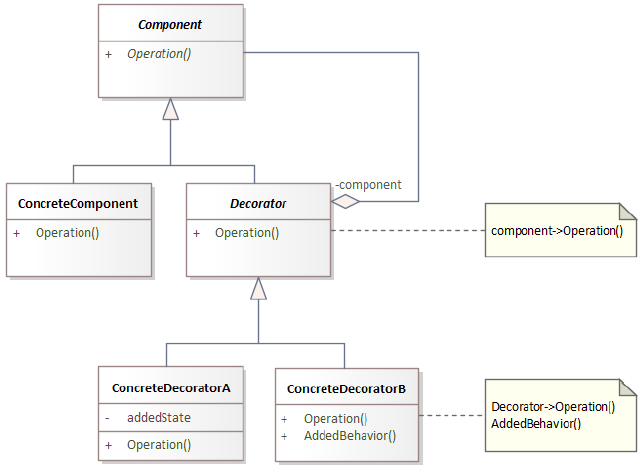
\includegraphics[width=0.8\linewidth]{../img/decorator_pattern.png}\\
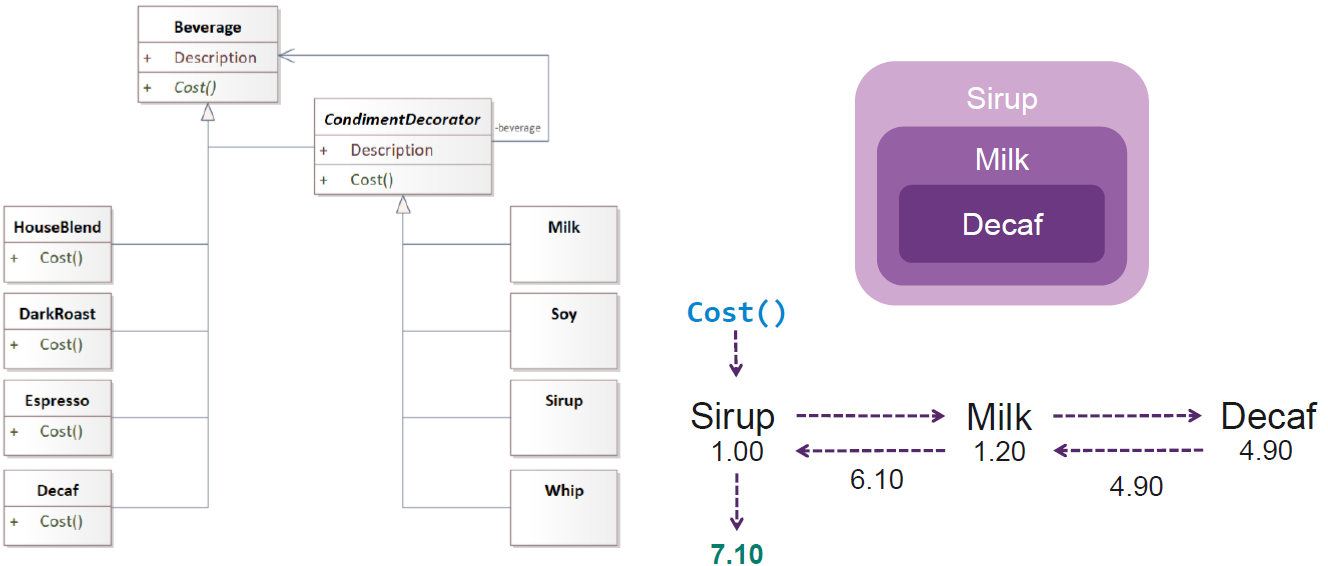
\includegraphics[width=\linewidth]{../img/decorator_pattern_2.png}\\
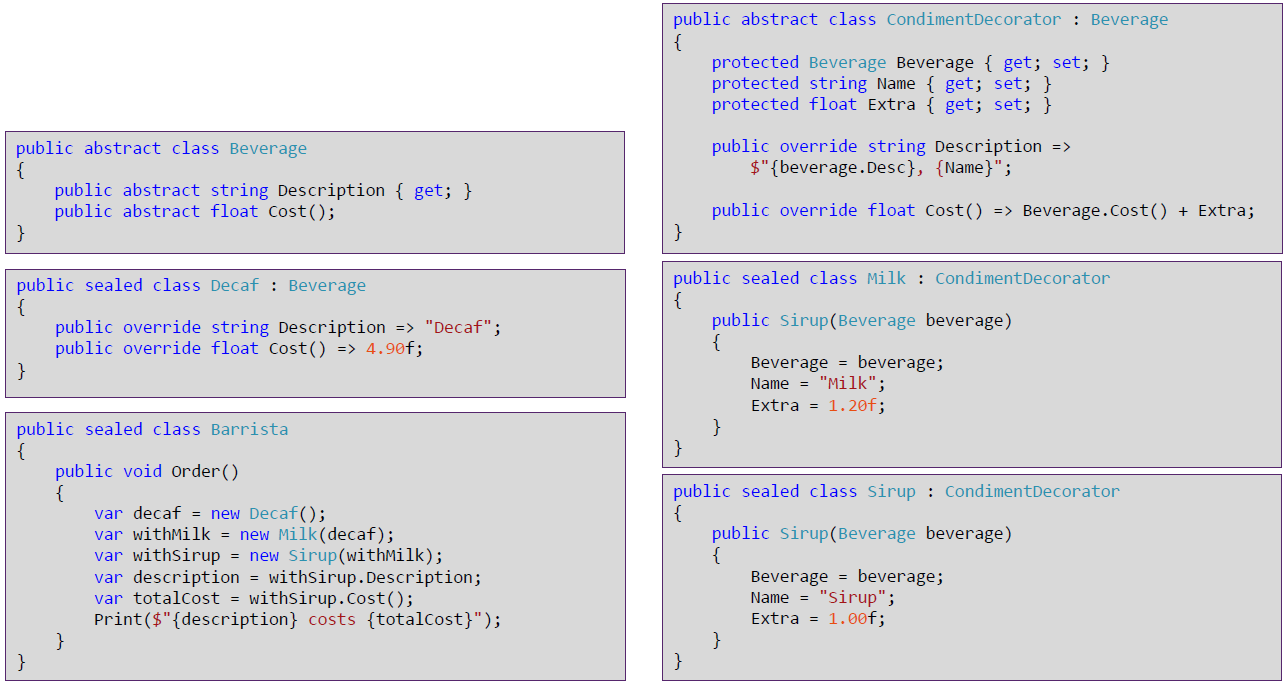
\includegraphics[width=\linewidth]{../img/decorator_pattern_code.png}\\

\subsection{Proxy}
Provide a surrogate or placeholder for another object to control access to it.\\
\begin{itemize}
    \item Often created within a Factory
    \item Controls access to the wrapped object
    \item Proxy and wrappee have the same interface
\end{itemize}
\textbf{Variations}
\begin{itemize}
    \item Virtual Proxy: access to an expensive to instantiate object
    \item Remote Proxy: interaction between a client and a remote object
    \item Protection Proxy: controls access to the original object
\end{itemize}
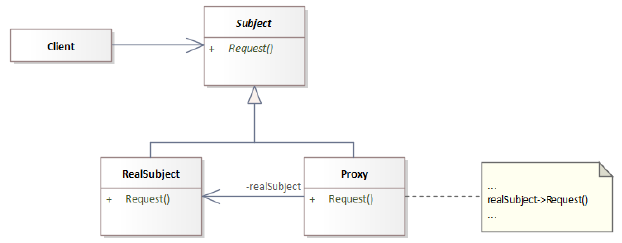
\includegraphics[width=0.8\linewidth]{../img/proxy_pattern.png}
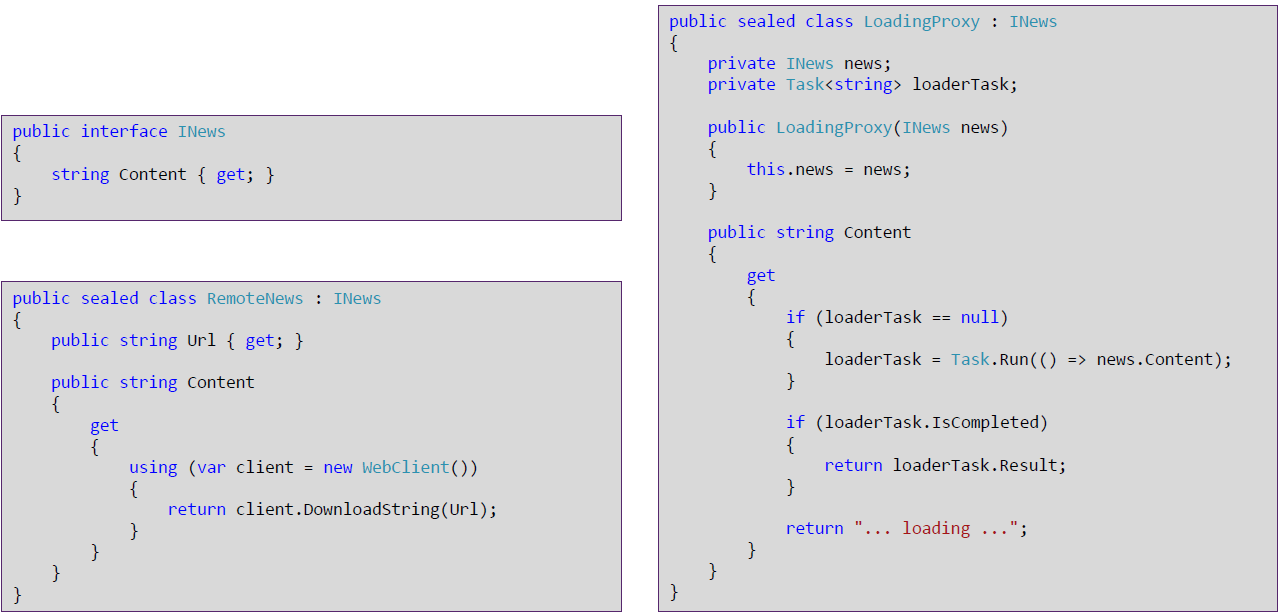
\includegraphics[width=\linewidth]{../img/proxy_pattern_code.png}

\subsection{Summary}
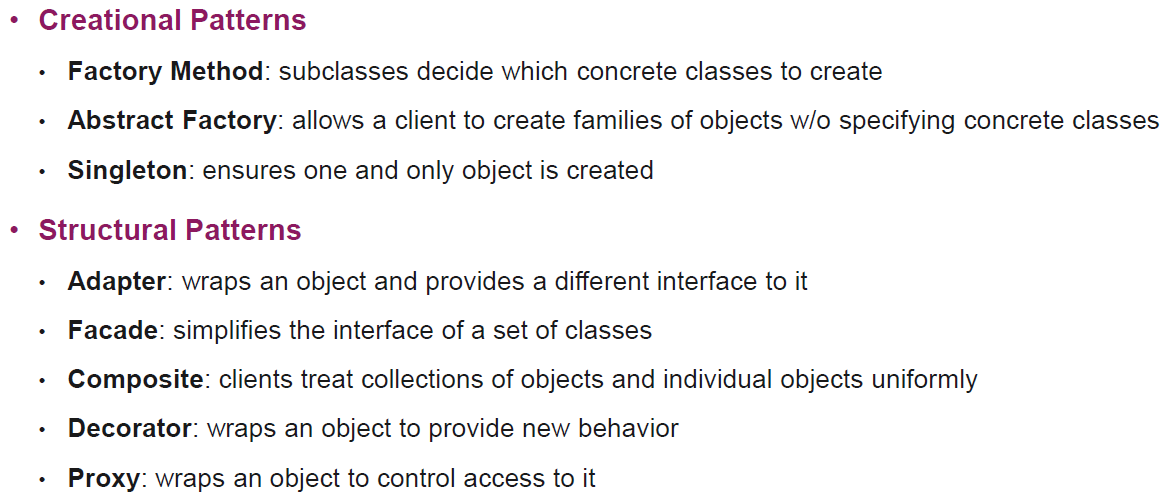
\includegraphics[width=\linewidth]{../img/patterns_summary.png}



        %! Author = Philipp Emmenegger
%! Date = 09/06/2021

\section{Refactoring}
\textbf{Reasons}
\begin{itemize}
    \item Programs, like people, get old
    \item Broken Windows
    \item Under / Over Engineering
    \item Technical Dept
\end{itemize}

\subsection{Definition}
\begin{itemize}
    \item Systematic approach
    \item Changes are based on a plan
    \item Improve the design of existing code
    \item Retain maintainability of code
    \item Make future changes easier
    \item No new features or functionality
    \item Software works same as before
\end{itemize}

\subsection{Benefits}
\begin{itemize}
    \item Improves the design of software
    \item Makes software easier to understand
    \item Helps to program faster
    \item Helps to find bugs
\end{itemize}

\subsection{Anatomy of a Refactoring}
\textbf{Name}
\begin{itemize}
    \item Builds a common vocabulary
    \item Same idea as giving names to Design Patterns
\end{itemize}
\textbf{Summary}
\begin{itemize}
    \item In which situation do you need it?
    \item What does it do?
\end{itemize}
\textbf{Motivation}
\begin{itemize}
    \item Why the refactoring should be done?
    \item When the refactoring should not be done?
\end{itemize}
\textbf{Mechanics}
\begin{itemize}
    \item How to carry out the refactoring?
    \item Concise, step-by-step description
\end{itemize}
\textbf{Optional sections}
\begin{itemize}
    \item Examples
    \item Inverse refactorings
\end{itemize}
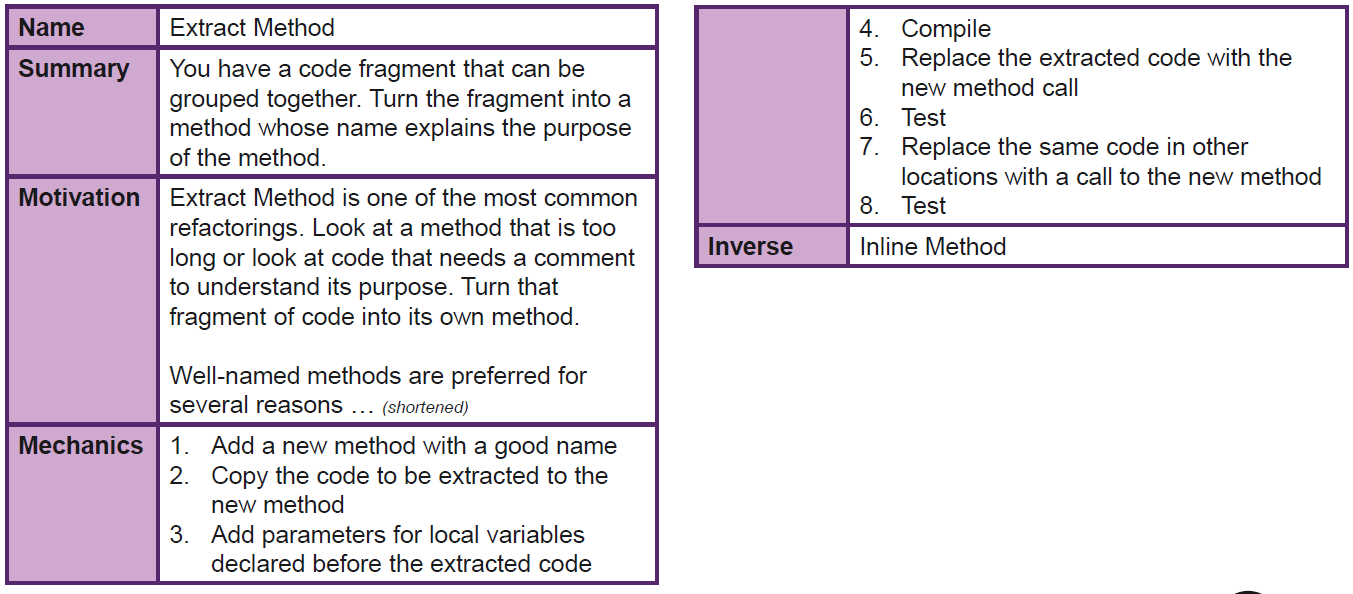
\includegraphics[width=\linewidth]{../img/refactoring_example.png}

\subsection{When to refactor?}
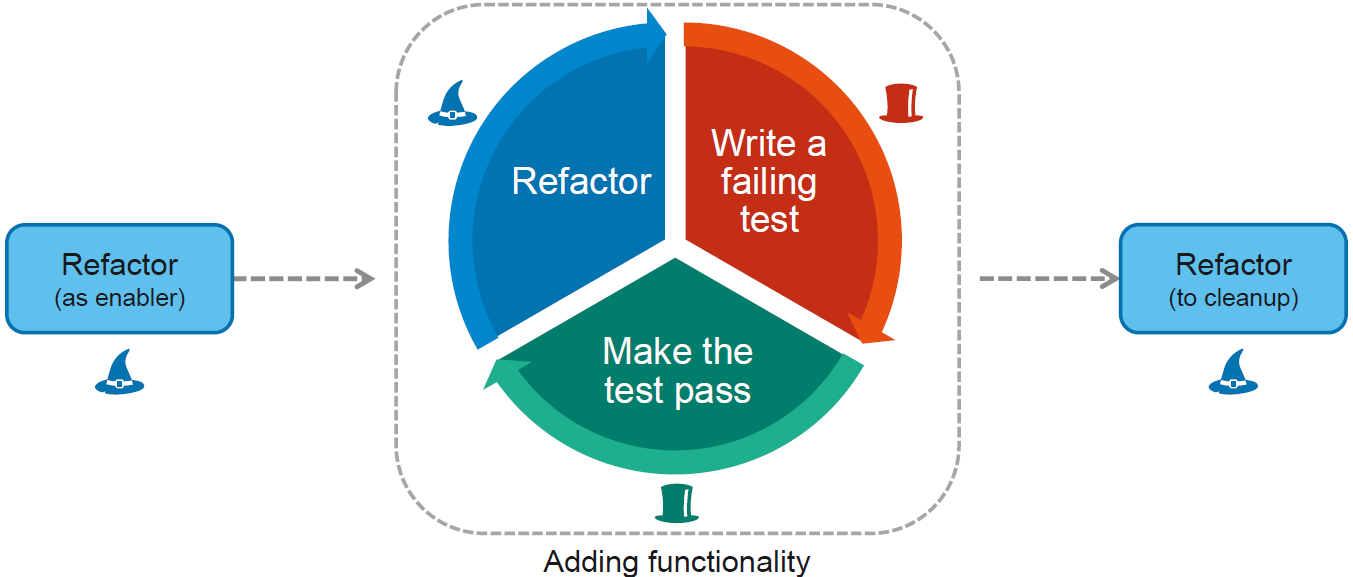
\includegraphics[width=\linewidth]{../img/refactoring_process.png}

\subsection{Code Smells}
\begin{itemize}
    \item Violate properties of Clean Code Principles
    \item Have names
    \item Easy to detect
    \item Have corresponding Refactorings
\end{itemize}
\textbf{Examples:}
\begin{itemize}
    \item Bloaters: Long Method, Large Class, Primitive Obsession..
    \item Object-Orientation Abusers: Switch Statements, Refused Bequest..
    \item Change Preventers: Divergent Change, Shotgun Surgery..
    \item Dispensables: Comments, Duplicated code, Dead Code..
    \item Couplers: Freature Envy, Inappropriate Intimacy..
\end{itemize}

\subsection{Anti Patterns}
\begin{itemize}
    \item Response to recurring problem that is ineffective or contra productive
    \item Have names
\end{itemize}
\textbf{Examples:}
\begin{itemize}
    \item Golden Hammer
    \item Not invented here (Belief that in-house is always better)
    \item Programming by Coincidence
    \item Big ball of mud (no structure)
\end{itemize}

\subsection{Legacy Code}
\begin{itemize}
    \item Valuable code devs are afraid to change
    \item Often lacks automated tests
    \item Contains Dependencies
\end{itemize}
\textbf{Dilemma}\\
When we change code, we should have tests in place. 
To put tests in place, we often have to change code.\\
\textbf{Dependencies}\\
One of the most critical problems in software development.\\
Much legacy code work involves breaking dependencies so that change can be easier.\\
\begin{itemize}
    \item 
\end{itemize}

\subsubsection{Legacy Code Change Algorithm}
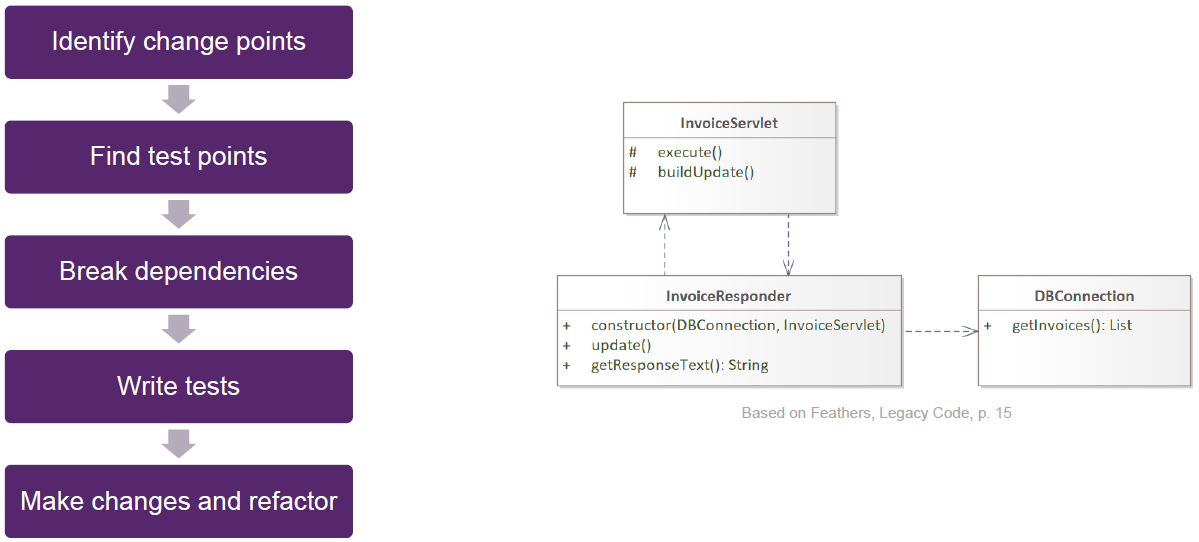
\includegraphics[width=\linewidth]{../img/legacy_code_change_algo.png}
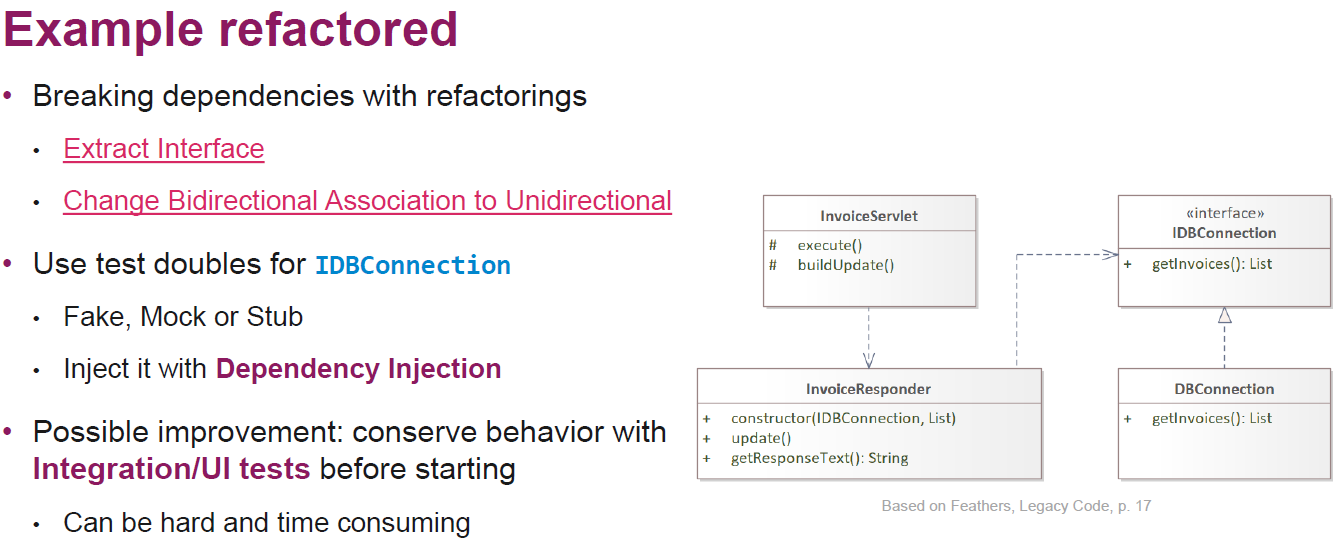
\includegraphics[width=\linewidth]{../img/legacy_code_change_algo_refactored.png}

\subsubsection{Extract and Override - Factory Method}
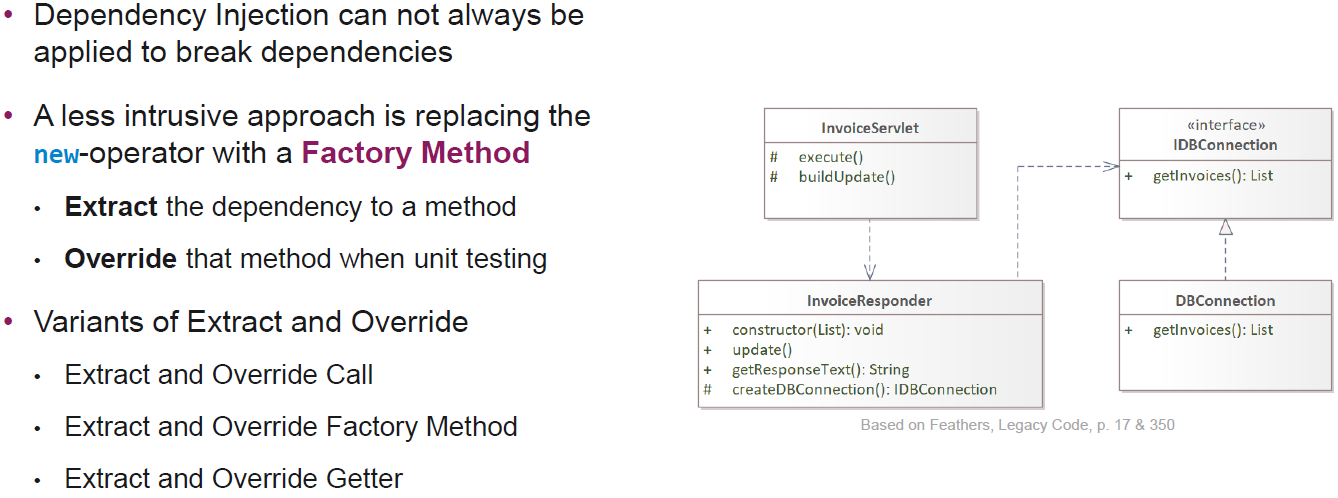
\includegraphics[width=\linewidth]{../img/extract_and_override.png}

\subsubsection{The Gilded Rose Kata}
\begin{enumerate}
    \item Understand the functionality
    \begin{itemize}
        \item Look out for Code Smells
        \item Gather ideas for a clean implementation
    \end{itemize}
    \item Preserve functionality with integration tests
    \item Refactor the existing code
    \item Implement new functionality (TDD Cycle)
\end{enumerate}
        %! Author = Philipp Emmenegger
%! Date = 09/06/2021

\section{Reviews}
\textbf{What to review:}
\begin{itemize}
    \item Requirements
    \item Architecture
    \item Design
    \item Usability
    \item Code
    \item Product
    \item Process
    \item Progress
    \item Collaboration
\end{itemize}
\textbf{Principles}
\begin{itemize}
    \item Timely
    \item Systematic
    \item Reasonable
\end{itemize}

\subsection{Techniques}
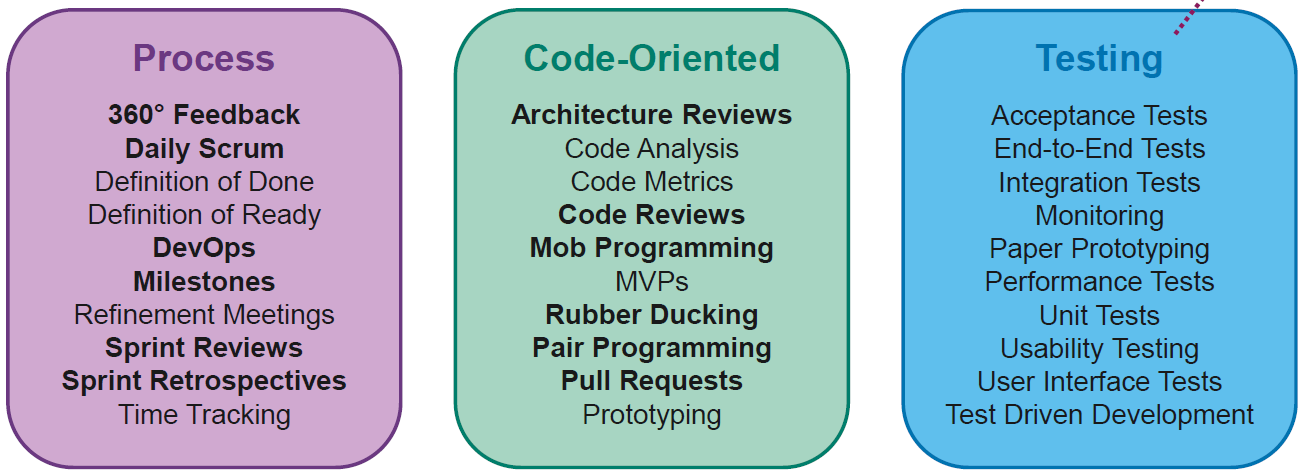
\includegraphics[width=\linewidth]{../img/review_techniques.png}

\subsubsection{Sprint Review}
\begin{itemize}
    \item ca. 1h per week
    \item Maybe start with presentation (state of project / goals / backlog / metrics)
    \item Involve the audience
    \item Attending the review should be fun
\end{itemize}

\subsubsection{Sprint Retrospective}
\begin{itemize}
    \item Communicate usefulness early and often
    \item Send invitations early / regularly
    \item Prepare materials in the room
    \item Repeat the rules before the meeting
    \item Findings should have impact on upcoming iterations
    \item Early in the project, go for quick wins
    \item Keep open impediments in a backlog
    \item Communicate progress
\end{itemize}
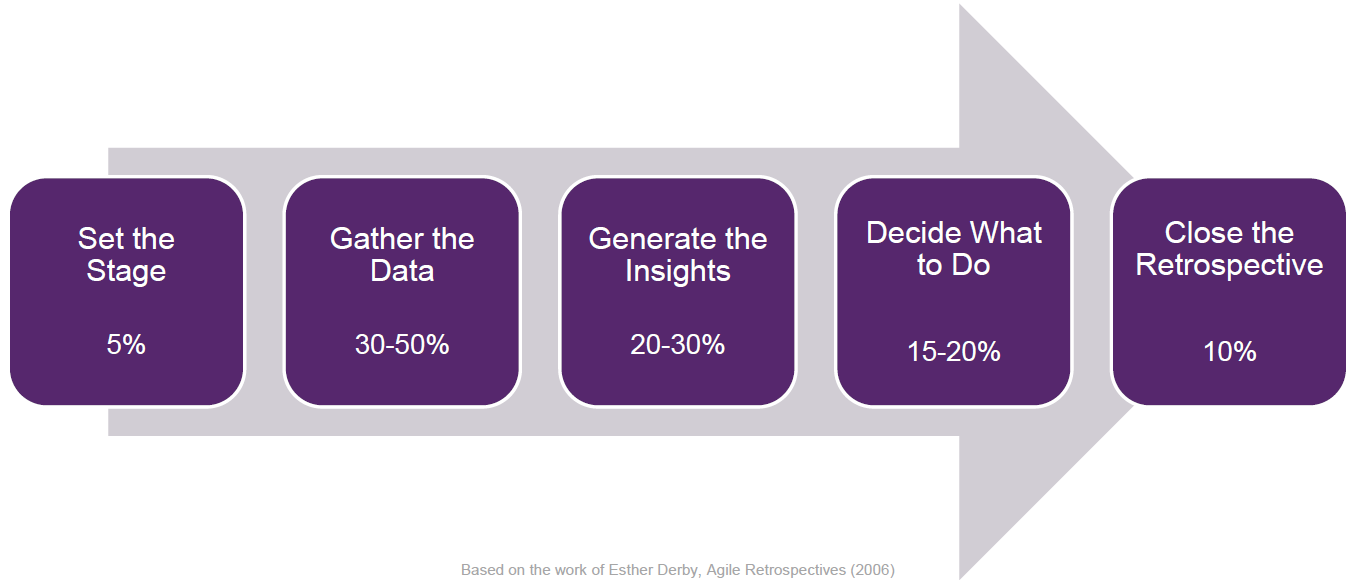
\includegraphics[width=\linewidth]{../img/sprint_retrospective.png}

\subsubsection{DevOps}
\includegraphics[width=0.7\linewidth]{../img/devops.png}

\subsubsection{360deg Feedback}
\begin{itemize}
    \item Incorporate results from different sources
    \item Self-assessment
    \item Manager
    \item Collaborators
    \item Customers
    \item Only works in an environment of trust
\end{itemize}

\subsection{Code-oriented Techniques}
\subsubsection{Rubber Ducking}
\textit{siehe clean coder oder so..}

\subsubsection{Pair Programming}
\textit{siehe clean coder oder so..}

\subsubsection{Mob Programming}
\begin{itemize}
    \item Pair programming with more attendees (Devs, Architects, Domain Experts...)
    \item Best suited for very difficult problems / mission critical parts of code
\end{itemize}

\subsubsection{Pull Requests}
\begin{enumerate}
    \item Dev makes changes on a branch
    \item Dev files a pull request
    \item Rest of the team reviews the code (check DoD)
    \item Maintainer merges into a stable branch
\end{enumerate}

\subsubsection{Code Reviews}
\begin{itemize}
    \item Formal way to assess code
    \item Performed manually, supported by tools
    \item Use it deliberately
\end{itemize}
\textbf{Roles}
\begin{itemize}
    \item Author
    \item Reviewer
    \item Moderator
    \item Recorder
    \item Attendee
\end{itemize}
\textbf{Artifacts}
\begin{itemize}
    \item Protocol
    \item Work Items (optional)
\end{itemize}
\textbf{Process:}
\includegraphics[width=\linewidth]{../img/code_reviews_process.png}
\textbf{Dos:}
\begin{itemize}
    \item Respect Feedback rules
    \item Only review code that satisfies DoD
    \item Choose appropriate amount of code
    \item As a reviewer, take your time
    \item Support the review with automated tools
    \item Use checklists
    \item Highlight positive examples
\end{itemize}
\textbf{Don'ts}
\begin{itemize}
    \item Fixing code during the review
    \item Never review simple code
    \item Do not invite people responsible for the author
\end{itemize}

\subsection{Architecture Reviews}
\begin{itemize}
    \item Quantitative: Metrics and Profiling
    \item Qualitative: Reviews ATAM
    \item combine the both!
\end{itemize}

\subsubsection{ATAM - Architecture Tradeoff Analysis Method}
\includegraphics[width=\linewidth]{../img/ATAM.png}
\includegraphics[width=\linewidth]{../img/ATAM_flow.png}


        %! Author = Philipp Emmenegger
%! Date = 09/06/2021

\section{Testing}
\subsection{Levels of Testing}
\includegraphics[width=\linewidth]{../img/levels_of_testing.png}
\textbf{Unit Tests}
\begin{itemize}
    \item Every unit is testet on its own
    \item All dependencies are broken using Test Doubles
    \item \textbf{FIRST}
    \begin{itemize}
        \item Fast
        \item Isolated
        \item Repeatable
        \item Self-Validating
        \item Timely
    \end{itemize}
    \item \textbf{AAA}
    \begin{itemize}
        \item Arrange
        \item Act
        \item Assert
    \end{itemize}
\end{itemize}
\textbf{Component Tests}
\begin{itemize}
    \item Complete components are tested
    \item Use doubles for dependencies outside of the component
\end{itemize}
\textbf{Integration Tests}
\begin{itemize}
    \item Use doubles for 'expensive' dependencies
    \item Communication between components is tested
\end{itemize}
\textbf{System Tests}
\begin{itemize}
    \item Test the full system
    \item Only use doubles if absolutely necessary
\end{itemize}

\subsection{Test Pyramid}
\includegraphics[width=\linewidth]{../img/test_pyramid.png}

\subsection{Environments}
\begin{itemize}
    \item DEV: Development and debugging
    \item TEST: Integration and System Tests
    \item STAGE: Acceptance Tests before releases
    \item PROD: Production
\end{itemize}
\textbf{Deployment}
\begin{itemize}
    \item DEV: On commits, pull requests, demand
    \item TEST: Every night from dev-branch
    \item STAGE: On demand before releases
    \item PROD: On demand on releases
\end{itemize}

\subsection{Integration and System Tests}
\textbf{Test Doubles}
 \begin{itemize}
     \item Pros: Faster, flexibility, less maintenance
     \item Cons: Not testing the reality (interfaces)
 \end{itemize}
\textbf{Environments}
\begin{itemize}
    \item Pros: Testing the reality
    \item Cons: Slower, less flexible, hard to maintain
\end{itemize}

\subsection{Alpha / Beta Testing}
\textbf{Alpha Testing}
\begin{itemize}
    \item Testing an early pre-release
    \item Some features might be missing
    \item Limited audience
    \item Find critical bugs before going public
\end{itemize}
\textbf{Beta Testing}
\begin{itemize}
    \item Testing the nearly finished product
    \item Feature-complete with focus on optimization
    \item Wide audience, typically external
    \item Test product within its productive environment
\end{itemize}

\subsection{Regression Testing}
\begin{itemize}
    \item Ensure that software still performs as expected after change
    \item If tests fail, that is called Regression
    \item Running unit tests after refactoring
    \item Running automated tests after a Sprint
\end{itemize}

\subsection{Performance Tests}
\begin{itemize}
    \item Manually using Integration / System tests
    \item Runtime
    \item Memory usage
    \item Power consumptions
    \item Impact of bad network quality
    \item Using Tools (Profiler)
\end{itemize}

\subsection{Monitoring}
\begin{itemize}
    \item Monitoring: Health of the system
    \item Analytics: What did the users do?
    \item Diagnostics: Where there any errors?
\end{itemize}

\subsection{A/B Testing}
\begin{itemize}
    \item User experience research methodology
    \item Compare two variants
    \item Determent which one is more effective
    \item Analytics data needed to rate efficiency
\end{itemize}

\subsection{Usability Testing}
\begin{itemize}
    \item Measure ease of use
    \item Testing product on users
    \item Observe users under controlled conditions
    \item Can be combined with A/B testing
\end{itemize}

\subsection{Paper Prototyping}
\begin{itemize}
    \item Test UI-Concepts
    \item Prototypes made from paper
    \item Helps understanding the requirements
\end{itemize}

    \end{multicols*}
\end{document}

























